\documentclass[a4paper,twoside,openleft]{blocksbook}
\usepackage[cm-default]{fontspec}% provides font selecting commands
\usepackage{xunicode}% provides unicode character macros
\usepackage{xltxtra} % provides some fixes/extras
\usepackage[answerdelayed,lastexercise]{exercise}
\usepackage[labelsep=period,labelfont=it,textfont=it]{caption}
\usepackage{alltt}
\usepackage{url}
\usepackage{listings} 
\usepackage{color}
\usepackage{graphicx}
\usepackage{relsize}
\usepackage{xCJK}
\usepackage{scalefnt}
\usepackage{wrapfig}
\usepackage{everypage}
% Tables from Gnumeric
\usepackage{array} 
\usepackage{longtable}
\usepackage{calc}
\usepackage{multirow}
\usepackage{hhline} 
\usepackage{ifthen} 
\usepackage{upquote}

\usepackage{tikz}
\usetikzlibrary{arrows,decorations.pathreplacing}
\usepackage{float}
\usepackage{coderemarks}    %% my own package

\defaultfontfeatures{Scale=MatchLowercase,Mapping=tex-text}
\setmainfont{Droid Serif}
\setsansfont{Droid Sans}
\setmonofont[SmallCapsFont={DejaVu Sans Mono},Scale=0.70]{DejaVu Sans Mono}
\def\inputGnumericTable{}

%% list of answers
\newlistof{listofex}{ex}{List of Exercises}
\newlistentry{exercise}{ex}{0}

%% does not work?
%% or \renewcommand*{\bibmark}{\markboth{\bibname}{}}
\renewcommand*{\bibmark}{\markboth{\bibname}{\bibname}}
\nobibintoc
\renewcommand*{\indexmark}{\markboth{\indexname}{\indexname}}
\noindexintoc
\makeindex

\expandafter\def\expandafter\quote\expandafter{\quote\em}

%%\DeclareCaptionFont{white}{\color{white}}
%%\DeclareCaptionFormat{listing}{\colorbox[cmyk]{0.43, 0.35,
%%0.35,0.01}{\parbox{0.5\textwidth}{\hspace{0.5em}#1#2#3}}} % 0.98 same as listings
%%\captionsetup[lstlisting]{format=listing,labelfont=white,textfont=white,singlelinecheck=false,margin=0em,font={bf,footnotesize}}

%% Listings
\lstdefinelanguage{Go}
  {morekeywords={break,cap,case,chan,const,continue,copy,default,defer,else,fallthrough,%
  for,func,go,goto,if,import,interface,len,make,map,new,package,range,return,select,%
  struct,switch,type,var,%  % types
  uint8,uint16,uint32,uint64,int8,int16,int32,int64,float32,float64,byte,%
  complex,complex32,complex64,%
  int,uint,float,bool,uintptr,string,%
  iota,%
  },%
  otherkeywords={<-,!,;,\{,\}},%  %% nog beter maken
    sensitive=true,%
    morecomment=[l]{//},%
    morecomment=[s]{/*}{*/},%
    morecomment=[n]{(*}{*)},%
    morestring=[b]",%
    morestring=[b]',%
  }[]%
\lstset{language=Go,inputencoding=utf8,extendedchars=false,texcl,escapechar=\|,basicstyle=\ttfamily,keywordstyle=\bfseries,numbers=none,numberblanklines=false,showstringspaces=false,breaklines=true,numberstyle=\tiny\ttfamily,xleftmargin=\parindent,xrightmargin=1em,linewidth=0.98\linewidth}

\renewcommand{\lstlistlistingname}{List of Go Code}
\newcommand{\coderemark}[1]{\qquad$\leftarrow \textit{\small #1}$}

%% Exercises
\renewcommand{\ExerciseHeaderTitle}{\ExerciseTitle}
\renewcommand{\ExerciseHeaderLabel}{}
\renewcommand{\ExerciseName}{}	%% was 'Exercise'
\renewcommand{\ExerciseHeaderNB}{\theExercise}
%% This one is actually used
\renewcommand{\ExerciseHeader}{\vspace{.7ex}\noindent\textbf{Q\theExercise}. (\number\ExerciseDifficulty) \ExerciseTitle\quad%
\addcontentsline{ex}{exercise}{\numberline{\theExercise}(\number\ExerciseDifficulty) \ExerciseTitle}}
\renewcommand{\AnswerHeader}{\vspace{.7ex}\noindent\textbf{A\theExercise}.  (\number\ExerciseDifficulty) \ExerciseTitle\quad}

%% Style commands
\newcommand{\func}[1]{\texttt{#1}}
\newcommand{\key}[1]{\texttt{\textbf{#1}}}
\newcommand{\type}[1]{\texttt{\textbf{#1}}}
\newcommand{\prog}[1]{\texttt{#1}}
\newcommand{\dir}[1]{\texttt{#1}}
\newcommand{\var}[1]{\texttt{#1}}
\newcommand{\rem}[1]{\texttt{\textit{#1}}}
\newcommand{\package}[1]{{\textit{#1}}}
\newcommand{\softnewline}{\Pisymbol{psy}{191}}
\newcommand{\hardnewline}{\ \\}
\newcommand{\first}[1]{\emph{#1}\index{#1}}
\newcommand{\second}[1]{#1\index{#1}}
\newcommand{\epi}[2]{\epigraph{#1}{#2}}
\newcommand{\hg}[1]{\newline{\texttt{\tiny{Go release.#1}}}}
\newcommand{\error}[1]{\texttt{#1}}

% Colors
\definecolor{gray20}{gray}{0.20}
\newcommand{\lgray}[1]{{\color{gray20}#1}}
\newcommand{\pr}{\lgray{\%}}

\newenvironment{display}{\def\FrameCommand{\hskip\parindent}%%
\MakeFramed{\advance\hsize-\width\FrameRestore}%%
\vspace*{-2ex}\small\begin{alltt}}%
{\end{alltt}\vspace*{-2ex}\endMakeFramed}

\newenvironment{lbar}{%
\def\FrameCommand{\rightskip=\parindent\hskip\parindent\vrule width 1pt \hspace{10pt}}%
\MakeFramed{\rightskip=\parindent\advance\hsize-\width \FrameRestore}}%
{\endMakeFramed}

%% Margin notes
\setmarginnotes{20pt}{80pt}{\onelineskip}
\newcommand{\gomarginpar}[1]{%
\marginpar{\sffamily#1}}
\newcommand{\todo}[1]{%
\marginpar{\sffamily{todo}\\#1}}
%% typeset text in margin and index arg 2
\newcommand{\gomarginindex}[2]{%
\gomarginpar{#1}\index{#2}}

\newenvironment{cjk}{%
\begin{CJK*}{UTF8}{song}
\setCJKfamilyfont{Japanese}{Sazanami Gothic}
\CJKfamily{Japanese}
}%
{%
\end{CJK*}%
}

%%%%%%%%%%%%%%%%%%%%%%%%%%%%%%%%%%%%%%%%%%%%%%%%%%%%%%%%%%%%%%%%
%% ccBeamer 0.1, 2007-07-02                                   %%
%% Written by Sebastian Pipping <webmaster@hartwork.org>      %%
%% ---------------------------------------------------------- %%
%% Licensed under Creative Commons Attribution-ShareAlike 3.0 %%
%% http://creativecommons.org/licenses/by-sa/3.0/             %%
%%%%%%%%%%%%%%%%%%%%%%%%%%%%%%%%%%%%%%%%%%%%%%%%%%%%%%%%%%%%%%%%


%% Images
\newcommand{\CcImageBy}[1]{%
	
\includegraphics[scale=#1]{creative_commons/cc_by_30.pdf}%
}
\newcommand{\CcImageCc}[1]{%
	
\includegraphics[scale=#1]{creative_commons/cc_cc_30.pdf}%
}
\newcommand{\CcImageDevNations}[1]{%
	
\includegraphics[scale=#1]{creative_commons/cc_dev_nations_30.pdf}%
}
\newcommand{\CcImageNc}[1]{%
	
\includegraphics[scale=#1]{creative_commons/cc_nc_30.pdf}%
}
\newcommand{\CcImageNd}[1]{%
	
\includegraphics[scale=#1]{creative_commons/cc_nd_30.pdf}%
}
\newcommand{\CcImagePd}[1]{%
	
\includegraphics[scale=#1]{creative_commons/cc_pd_30.pdf}%
}
\newcommand{\CcImageSa}[1]{%
	
\includegraphics[scale=#1]{creative_commons/cc_sa_30.pdf}%
}
\newcommand{\CcImageSampling}[1]{%
	
\includegraphics[scale=#1]{creative_commons/cc_sampling_30.pdf}%
}
\newcommand{\CcImageSamplingPlus}[1]{%
	
\includegraphics[scale=#1]{creative_commons/cc_sampling_plus_30.pdf}%
}


%% Groups
\newcommand{\CcGroupBy}[1]{% zoom
	\CcImageBy{#1}%
}
\newcommand{\CcGroupByNc}[2]{% zoom, gap
	\CcImageBy{#1}\hspace*{#2}\CcImageNc{#1}%
}
\newcommand{\CcGroupByNcNd}[2]{% zoom, gap
	\CcImageBy{#1}\hspace*{#2}\CcImageNc{#1}\hspace*{#2}\CcImageNd{#1}%
}
\newcommand{\CcGroupByNcSa}[2]{% zoom, gap
	\CcImageBy{#1}\hspace*{#2}\CcImageNc{#1}\hspace*{#2}\CcImageSa{#1}%
}
\newcommand{\CcGroupByNd}[2]{% zoom, gap
	\CcImageBy{#1}\hspace*{#2}\CcImageNd{#1}%
}
\newcommand{\CcGroupBySa}[2]{% zoom, gap
	\CcImageBy{#1}\hspace*{#2}\CcImageSa{#1}%
}
\newcommand{\CcGroupDevNations}[1]{% zoom
	\CcImageDevNations{#1}%
}
\newcommand{\CcGroupNcSampling}[2]{% zoom, gap
	\CcImageNc{#1}\hspace*{#2}\CcImageSampling{#1}%
}
\newcommand{\CcGroupPd}[1]{% zoom
	\CcImagePd{#1}%
}
\newcommand{\CcGroupSampling}[1]{% zoom
	\CcImageSampling{#1}%
}
\newcommand{\CcGroupSamplingPlus}[1]{% zoom
	\CcImageSamplingPlus{#1}%
}


%% Text
\newcommand{\CcLongnameBy}{Attribution}
\newcommand{\CcLongnameByNc}{Attribution-NonCommercial}
\newcommand{\CcLongnameByNcNd}{Attribution-NoDerivs}
\newcommand{\CcLongnameByNcSa}{Attribution-NonCommercial-ShareAlike}
\newcommand{\CcLongnameByNd}{Attribution-NoDerivs}
\newcommand{\CcLongnameBySa}{Attribution-ShareAlike}

\newcommand{\CcNote}[1]{% longname
	This work is licensed under the \textit{Creative Commons #1 3.0 License}.%
}

%%\input{draft.tex}
%%\AddEverypageHook{\pagedraft}
%%\usepackage{refcheck}
%% a5paper
%\setlength{\voffset}{-0.10\stockheight} 
%\addtolength{\textheight}{0.12\stockheight}

\begin{document}
\thispagestyle{empty}
\newcommand{\version}{0.3}
%% Title page
\begin{figure}[t!]
\begin{center}
    \hspace{1.0cm}{\scalefont{6.00}{\sffamily{\mbox{\vspace{1.0cm}Learning Go}}}}
    \includegraphics[scale=0.65]{fig/bumper-inverse.png}
\end{center}
\end{figure}
\vspace*{0.02\stockheight}
\begin{minipage}{0.4\textwidth}
\begin{flushleft} \large
\hspace*{2,0cm}Authors:\\
\hspace*{2.0cm}\emph{Miek Gieben}\\
%%\hspace*{2.0cm}\emph{JC van Winkel}\\
%%\hspace*{2.0cm}\emph{Jeroen Bulten}\\
\vfill
\end{flushleft}
\end{minipage}
\hspace{5mm}
\begin{minipage}{0.4\textwidth}
\begin{flushright} \large
Thanks to:\\
\emph{Go Authors}\\
\emph{Google}\\
\emph{Go Nuts mailing list}\\
\vfill
\end{flushright}
\end{minipage}
\vfill
\begin{center}
    \hspace*{1cm}\CcGroupByNcSa{0.83}{0.95ex}\\[2.5ex]
    \hspace*{1cm}{\tiny\CcNote{\CcLongnameByNcSa}}
\newline\hspace*{1cm}{\tiny Build: \version --- \today}
\end{center}
\vspace{-3em}
%% End title page %%

\newpage

\thispagestyle{empty}
\begin{figure}[H]
\begin{center}
%%PDFcrop fails on Ubuntu
%%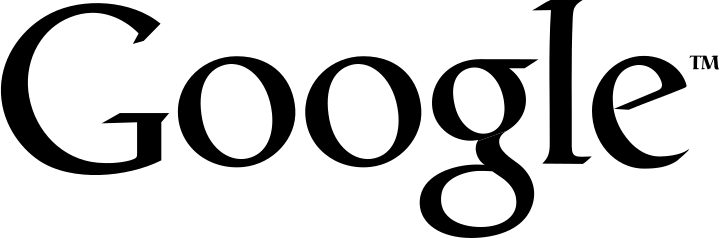
\includegraphics[scale=0.50]{fig/google_logo_black.pdf}
\end{center}
\end{figure}
\begin{center}
\vfill
\emph{Learning as we Go.}

\emph{\tiny{Updated to Go \gorelease{2010-10-20}.}}
\vspace{.2\stockheight}
\end{center}

\clearpage

\pagenumbering{roman}
\tableofcontents*
\listoffigures*
\listoftables*
\listofcode* 
\listofex* 
\clearpage

%% \section{To do}

\begin{itemize}
Run gotest -test.bench=Bench -test.cpuprofile=cpuprof

This will generate a cpu profile. You can examine it with gopprof:

gopprof 8.out cpuprof

- Evan

\item
Style! Make it a pleasant read
\item
In chapter 3 (Functions) add exercise for GCD and LCM
\item
Conversion 
\end{itemize}
Exercise ideas
\begin{itemize}
\item
sudoku solver
\item
concurrent/parallel Sudoku solver
\item
prime number tester
\item
prime number generator
\item
prime sieve
\item
get system time and convert it in different formats:
\item
Extract uppercase words from a file
\end{itemize}

%% \part{Learning Go} %%

\chapter{Introduction}
\label{chap:intro}
\epi{``对此感兴趣,并且希望做点什么。''}
{\textit{在为 Go 添加复数支持时}\\ \textsc{KEN THOMPSON}}

\noindent{}什么是 Go?来自其网站\cite{go_web}的介绍:
\begin{quote}
Go 编程语言是一个使得程序员更加有效率的开源项目。Go 是有表达力、简洁、清晰和有效率的。
它的并行机制使其很容易编写多核和网络应用,而新奇的类型系统允许构建有弹性的模块化程序。
Go 编译到机器码非常快速,同时具有便利的垃圾回收和强大的运行时反射。
它是快速的、静态类型编译语言,但是感觉上是动态类型的,解释型语言。
\end{quote}

Go 1 是 Go 语言的第一个稳定发布版本。
本文档的所有练习都工作于 Go 1 —— 如果不行,那就是 bug。

本书使用了下面的约定:
\begin{itemize}
\item 代码用 \prog{DejaVu Mono} 显示;
\item 关键词用 \key{DejaVu Mono Bold} 显示;
\item 注释用 \rem{DejaVu Mono Italic} 显示;
\item 代码中额外的标记,\coderemark{用这种形式展现};
\item 使用数字 \gocircle{1} 对长内容标记——解释会跟随其后;
\item 行号在右边展示;
\item Shell 示例用 \pr{} 作为标记;
\item 强调的段落会缩进,在左边有竖线。
\end{itemize}

\section{官方文档}
Go 已经有大量的文档。
\gomarginpar{在互联网上搜索时,应当使用``golang''这个词来代替原始的``go''。}
例如 Go Tutorial \cite{go_tutorial} 和 Effective Go \cite{effective_go}。
网站 \url{http://golang.org/doc/} 是绝佳的起点 
\footnote{\url{http://golang.org/doc/} 本身是由 Go 程序 \prog{godoc} 提供服务的。}。
虽然并不一定要阅读这些文档,但是强烈建议这么做。

Go 1 可以用两个程序提供文档服务:
\begin{enumerate}
\item \prog{go doc},该程序用于(第三方)\emph{包}文档;
\item \prog{godoc},用于官方包文档,例如 Go 1 相关的所有内容。
\end{enumerate}

这两个最明显的区别在于内建文档(参阅下一章的``\titleref{sec:builtins}``):
\begin{display}
\pr \user{go doc builtin}   \coderemark{35 lines}
\pr \user{godoc builtin}    \coderemark{242 lines}
\end{display}

通常这两个的区别并无大碍,不过要留意 
\prog{go doc} 和 \prog{godoc} 并不等同。
在第 \ref{chap:packages} 章解释了如何构造你自己的包的文档。

\section{前身}
Go 的前身来自于 Inferno \cite{inferno} (基于 Plan 9 \cite{plan9} 的改造)。
Inferno 包含了一个叫做 Limbo \cite{limbo} 的语言。这里引用了一段来自于 Limbo 论文的描述:
\begin{quote}
Limbo 是用于开发运行在小型计算机上的分布式应用的编程语言。
它支持模块化编程,编译期和运行时的强类型检查,\emph{进程内基于具有类型的 channel 通讯},
原子性\emph{垃圾收集},和简单的抽象数据类型。
它被设计用于即便是没有硬件内存保护的小型设备上,也能安全的运行。
\end{quote}
Go 从 Limbo 继承的另一个特性是 channel(参阅第 \ref{chap:channels} 章)。
从 Limbo 文档来的另一段描述:
\begin{quote}
[channel] 是用于向系统中其他代理发送和接收特定类型对象的通讯机制。
channel 可以用于本地进程间通讯;用于连接到命名的目的地的库方法。
两种情况都是直接发送和接收操作的。
\end{quote}
在 Go 中,channel 比在 Limbo 中更加好用。
如果我们对 Go 的历史深入探索,会发现一个到 ``Newsqueak'' \cite{newsqueak} 的引用,
这是在类 C 语言中使用 channel 通讯的拓荒者。
channel 对于这些语言并不是独一无二的,另一个非类 C 语言,Erlang \cite{erlang},也在使用它。

\begin{figure}[H]
\caption{Go 编年史}
\label{fig:chrono-of-go}
\begin{center}
\includegraphics[scale=0.65]{fig/go-history.pdf}
\end{center}
\end{figure}

使用 channel 与其他进程进行通讯的办法,
叫做通讯序列化过程(Communicating Sequential Processes - CSP),
由 C. A. R. Hoare \cite{hoare} 设计构想,而他正是那个发明快速排序 \cite{quicksort} 算法的人。

\begin{lbar}[]
Go 是第一个实现了简单的(或更加简单的)并行开发的、跨平台类 C 语言。
\end{lbar}

\section{获得 Go}
在这一节中将介绍如何在本地设备上安装 Go,不过也可以在线上的 \url{http://play.golang.org/} 编译 Go 代码。这是最为便捷的尝试代码的方法。

也可以从网站\cite{go_install}获得已经编译好的二进制版本。

Ubuntu 和 Debian 在其仓库中都有 Go 包,可以查找``golang''包。
但是工作的时候会有一些小问题。所以现在仍然使用源码进行安装。

因此只能手工从 mercurial 中获取 Go 代码并且编译。
对于其他类 Unix 系统,过程类似。
\begin{itemize}
\item 首先安装 Mercurial (获取 \prog{hg} 命令)。
在 Ubuntu/Debian/Fedora 需要安装 \prog{mercurial} 包;

\item 为了编译 Go 需要包:\prog{bison},\prog{gcc},\prog{libc6-dev},\prog{ed},\prog{gawk} 和 \prog{make};

\item 设置环境变量 \prog{GOROOT} 为 Go 安装目录:
\begin{display}
\pr \user{export GOROOT=\~{}/go}
\end{display}

\item 然后获取 Go 最新的发布版(=Go 1)源代码:
\begin{display}
\pr \user{hg clone -r release https://go.googlecode.com/hg/ \$GOROOT}
\end{display}

\item 设置 PATH 到 Go 的二进制文件所在目录,这样 Shell 可以找到它们:
\begin{display}
\pr \user{export PATH=$GOROOT/bin:$PATH}
\end{display}

\item 编译 Go
\begin{display}
\pr \user{cd \$GOROOT/src}
\pr \user{./all.bash}
\end{display}
\end{itemize}
如果全部都没问题,你最终会看到下面的内容:
\begin{display}
+--- cd ../test
+0 known bugs; 0 unexpected bugs
+
+ALL TESTS PASSED
+
+---
+Installed Go for linux/amd64 in /home/go
+Installed commands in /home/go/bin
\end{display}

\section{在 Windows 下获得 Go}

最好的方式是遵从网站\cite{go_install}的介绍,为了方便重复如下。

\begin{itemize}
\item 下载 Go -1:
\url{http://code.google.com/p/go/downloads/list?q=OpSys-Windows+Type%3DArchive};
\item 解压缩到 \verb|C:\| 盘;
\item 确保内容在 \verb|C:\Go|。注意:在解压缩 zip 文件时,这个目录会被创建;
\item 添加 \verb|C:\Go\bin| 到 \$PATH:
\begin{display}
export PATH=\verb|C:\Go\bin|
\end{display}
\end{itemize}

\section{练习}
\begin{Exercise}[title={Documentation},difficulty=1]
\label{ex:doc}
\Question
Go 的文档可以通过 \prog{godoc} 程序阅读,它包含在 Go 的发布包中。

\prog{godoc hash} 给出了 \package{hash} 包的信息。
阅读 \package{container} 包的帮助,给出了下面的结果:
\vskip\baselineskip
\begin{display}
SUBDIRECTORIES

heap
list
ring
vector
\end{display}
\vskip\baselineskip
哪个 \prog{godoc} 的命令可以显示 \package{container} 包中的 \package{vector} 文档?

\end{Exercise}

\begin{Answer}
\Question
\package{vector} 包在 \package{container} 的\emph{子目录}中,所以只需要 \quad \texttt{godoc
container/vector} 即可。

也可以指定“Go 手册”中某个函数的的文档。例如,函数
\func{Printf} 在 \package{fmt} 包中,仅阅读这个函数的文档,使用:\prog{godoc fmt Printf}{}。

甚至可以显示源代码:\prog{godoc -src fmt Printf}。
\end{Answer}


\cleardoublepage
\section{答案}
\shipoutAnswer


\chapter{Basics}
\pagenumbering{arabic}
\label{chap:basics}
\epi{``I am interested in this and hope to do something.''}
{\textit{On adding complex numbers to Go}\\ \textsc{KEN THOMPSON}}

\noindent{}What is Go? From the website \cite{go_web}:
\begin{quote}
The Go programming language is an open source project to make
programmers more productive. Go is expressive, concise, clean, and
efficient. Its concurrency mechanisms make it easy to write programs
that get the most out of multi core and networked machines, while its
novel type system enables flexible and modular program construction. Go
compiles quickly to machine code yet has the convenience of garbage
collection and the power of run-time reflection. It's a fast, statically
typed, compiled language that feels like a dynamically typed,
interpreted language.
\end{quote}

Go 1 is the first stable release of the language Go. 
This document and all exercises work with Go 1 -- if not, it's a bug.

The following convention is used throughout this book:
\begin{itemize}
\item Code, keywords and comments are displayed in \prog{Source Code Pro};
\item Extra remarks in the code \coderemark{Are displayed like this};
\item Longer remarks get a number -- \gocircle{1} -- with the explanation following;
\item Line numbers (if needed) are printed on the right side;
\item Shell examples use a \pr{} as prompt;
\item User entered text in shell examples \texttt{\user{is in bold}}, system responses
are in a \texttt{plain bold font};
\item An emphasized paragraph is indented and has a vertical bar on the
left.
\end{itemize}

\section{Official documentation}
There is already a substantial amount of documentation written about Go.
\gomarginpar{When searching on the internet use the term ``golang'' instead of plain ``go''.}
The Go Tutorial \cite{go_tutorial}, and the Effective Go
document \cite{effective_go}. The
website \url{http://golang.org/doc/} is a very good starting point
for reading up on Go\footnote{\url{http://golang.org/doc/} itself is served by 
\prog{go doc}.}. Reading these documents is
certainly not required, but it is recommended.

Go 1 comes with its own documentation in the form of a program called 
\prog{go doc}. If you are interested in the documentation
for the built-ins (see ``\titleref{sec:builtins}'' in the next chapter) you
can fire it up, like so:
\begin{display}
\pr \user{go doc builtin}
\end{display}

How to create your own package documentation is explained in chapter \ref{chap:packages}.

There are a few things that make Go different from other languages.
\begin{description}
\item[Clean and Simple]
Go strives to keep things small and beautiful. You should
be able to do a lot in only a few lines of code;

\item[Concurrent]
Go makes it easy to ``fire off'' functions to be
run as \emph{very} lightweight threads. These threads are called
\first{goroutines}{goroutines} \footnote{Yes, that sounds a lot like
\emph{co}routines, but goroutines are slightly different as we will
see in chapter \ref{chap:channels}.} in Go;

\item[Channels] 
Communication with these goroutines is done
via \first{channels}{channels} \cite{csp, hoare};

\item[Fast]
Compilation is fast and execution is fast. The aim is
to be as fast as C. Compilation time is measured in seconds;

\item[Safe]
Explicit casting and strict rules when converting one type to another.
Go has garbage collection, no more \func{free()} in Go, the language takes care of this;

\item[Standard format]
A Go program can be formatted in (almost) any way the programmers want,
but an official format exists. The rule is very simple:
The output of the filter \prog{gofmt} \emph{is the officially endorsed
format}.

\item[Postfix types]
Types are given \emph{after} the variable name, thus \prog{var a int},
instead of \prog{int a;} as one would in C;

\item[UTF-8]
UTF-8 is everywhere, in strings
\emph{and} in the program code. Finally you can use \prog{$\Phi$ =
$\Phi$ + 1} in your source code;

\item[Open Source]
The Go license is completely open source, see the file LICENSE in the Go
source code distribution;

\item[Fun]
Programming with Go should be fun!
\end{description}
Erlang \cite{erlang} also shares some
of the features of Go. Notable differences between Erlang
and Go is that Erlang borders on being a functional language,
where Go is an imperative one. And Erlang runs in a virtual
machine, while Go is compiled. Go also has a much more Unix-like
feel to it.

\begin{lbar}[]
Go is the first C--like language that is widely available,
runs on many different platforms and makes concurrency easy (or easier).
\end{lbar}

\section{Hello World}
\label{sec:hello world}
In the Go tutorial, Go is presented to the world in the typical
manner: letting it print ``Hello World'' (Ken Thompson and
Dennis Ritchie started this when they presented the C language in 
the 1970s). We don't think we can do better, so
here it is, ``Hello World'' in Go.

\lstinputlisting[label=src:hello,caption=Hello world]{src/helloworld.go}
Lets look at the program line by line.
\showremarks

\section{Compiling and running code}
\label{sec:building a program}
The preferred way to build a Go program is to use the \prog{go} tool.\index{tooling!go}
To build \prog{helloworld} we just enter:
\begin{display}
\pr \user{go build helloworld.go}
\end{display}
\index{tooling!go!build}
This results in an executable called \prog{helloworld}.

\begin{display}
\pr \user{./helloworld}
\end{display}

\vspace{-3.0ex}
\texttt{Hello, world; or }%
\begin{math}\kappa\alpha\lambda\eta\mu\acute{\epsilon}\rho\alpha\hspace{1em}\kappa\end{math}%
\'o\begin{math} \sigma\mu\epsilon\end{math}\texttt{; or }こんにちは 世界
\ \newline
\ \newline

\section{Settings used in this book}
\label{sec:settings_used}
\begin{itemize}                            
\item Go itself is installed in \file{\~{}/go}, and \var{\$GOROOT} is set to \var{GOROOT=\~{}/go} ;     
\item Go source code we want to compile ourself is placed in \file{\~{}/g/src} and
\var{\$GOPATH} is set to \var{GOPATH=\~{}/g} . This variable comes into play
when we start using packages (chapter \ref{chap:packages}).
\end{itemize}

\section{Variables, types and keywords}
\label{sec:vars}
In the next few sections we will look at the variables, basic types,
keywords and control structures of our new language. 
Go has a C-like feel when it comes to its syntax. 
If you want to put two (or more) statements on one line, they must be
separated with a semicolon (';'). Normally you don't need the semicolon.

Go is different from other languages in that the type of a variable
is specified \emph{after} the variable name. So not: 
\lstinline{int a}, but \lstinline{a int}. When declaring a variable it
is assigned the ``natural'' null value for the type. This means that after
\lstinline{var a int}, \lstinline{a} has a value of 0. With
\lstinline{var s string}, \lstinline{s} is assigned the zero string,
which is \lstinline{""}. 

Declaring and assigning in Go is a two step process, but they may
be combined. Compare the following pieces of code which have
the same effect. 
\index{variables!declaring}
\index{variables!assigning}

\begin{minipage}{.5\textwidth}
\begin{lstlisting}[linewidth=.5\textwidth,caption={Declaration with =}]
var a int
var b bool
a = 15
b = false
\end{lstlisting}
\hfill
\end{minipage}
\begin{minipage}{.5\textwidth}
\begin{lstlisting}[linewidth=.5\textwidth,caption={Declaration with :=}]
a := 15
b := false
\end{lstlisting}
\ \\
\ \\
\hfill
\end{minipage}

On the left we use the
\key{var} keyword to declare a variable and \emph{then} assign a value to
it. The code on the right uses \mbox{\key{:=}{ }} to do this in one
step (this form may only be used \emph{inside} functions).
In that case the variable
type is \emph{deduced} from the value. A value of 15 indicates an \type{int},
a value of \texttt{false} tells Go that the type should be \type{bool}. 
Multiple \key{var} declarations may also be grouped; \key{const}
and \key{import} also allow this. Note the use of parentheses:
\begin{lstlisting}
var (
    x int
    b bool
)
\end{lstlisting}
Multiple variables of the same type can also be declared on a
single line: \lstinline{var x, y int} makes \var{x} and \var{y} both
\type{int} variables. You can also make use of \first{parallel
assignment}{parallel assignment}:
\begin{lstlisting}
a, b := 20, 16
\end{lstlisting}
Which makes \var{a} and \var{b} both integer variables and assigns
20 to \var{a} and 16 to \var{b}.

A special name for a variable is \var{\textbf{\_}} \index{variables!\_}
(underscore)\index{variables!underscore}. Any value
assigned to it is discarded. In this example we only assign the integer
value of 35 to \var{b} and discard the value 34.
\begin{lstlisting}
_, b := 34, 35
\end{lstlisting}
Declared but otherwise unused variables are a compiler error in Go. The
following code generates this error:
\error{i declared and not used}

\begin{lstlisting}
package main
func main() { 
    var i int
}
\end{lstlisting}

\subsection{Boolean types}
A boolean type represents the set of boolean truth values denoted by the
predeclared constants \emph{true} and \emph{false}. The boolean type is \type{bool}.

\subsection{Numerical types}
Go has the well known types such as \lstinline{int}. This type
has the appropriate length for your machine,
meaning that on a 32-bit machine it is 32 bits and on
a 64-bit machine it is 64 bits. Note: an \lstinline{int} is
either 32 or 64 bits, no other values are defined. Same goes 
for \lstinline{uint}.

If you want to be explicit about the length you can have
that too with \lstinline{int32}, or \lstinline{uint32}. The full
list for (signed and unsigned) integers is
\type{int8}, \type{int16}, \type{int32}, \type{int64} and
\type{byte}, \type{uint8}, \type{uint16}, \type{uint32}, \type{uint64}.
With \lstinline{byte} being an
alias for \lstinline{uint8}. For floating point values there is
\lstinline{float32} and \lstinline{float64} (there is no \lstinline{float} type). 
A 64 bit integer or floating point value is \emph{always} 64 bit, also on 32 bit
architectures.

Note however
that these types are all distinct and assigning variables which mix
these types is a compiler error, like in the following code:
\lstinputlisting[numbers=right,label=src:types,caption=Familiar types are still distinct]{src/types.go}
Gives the error on the assignment on line 7:

\noindent\error{types.go:7: cannot use a + a (type int)  as type int32 in assignment}

The assigned values may be denoted using octal, hexadecimal or the scientific notation:
\lstinline{077}, \lstinline{0xFF}, \lstinline{1e3} or
\mbox{\lstinline{6.022e23}} are all valid.

\subsection{Constants}
\label{sec:constants}
Constants in Go are just that --- constant. They are created at compile
time, and can only be numbers, strings or booleans;
\lstinline{const x = 42} makes \var{x} a constant. You can use
\first{\key{iota}}{keyword!iota} \footnote{The word [iota] is used in a common English phrase,
'not one iota', meaning 'not the slightest difference', in reference to
a phrase in the New Testament: ``\emph{until heaven and earth pass away, not an
iota, not a dot, will pass from the Law}.'' \cite{iota}}
to enumerate values.
\begin{lstlisting}
const (
	a = iota
	b = iota 
)
\end{lstlisting}
The first use of \key{iota} will yield 0, so \var{a} is equal to 0, whenever
\key{iota} is used again on a new line its value is incremented with 1, so \var{b}
has a value of 1.

You can even do the following, let Go repeat the use of \key{= iota}:
\begin{lstlisting}
const (
	a = iota
	b	    |\coderemark{Implicitly \texttt{b = iota}}|
)
\end{lstlisting}
You may also explicitly type a constant, if you need that:
\begin{lstlisting}
const (
	a = 0           |\coderemark{Is an \key{int} now}|
	b string = "0" 
)
\end{lstlisting}

\subsection{Strings}
Another important built-in type is \lstinline{string}. Assigning a
string is as simple as:
\begin{lstlisting}
s := "Hello World!"
\end{lstlisting}
Strings in Go are a sequence of UTF-8 characters enclosed in double
quotes ("). If you use the single quote (') you mean one character
(encoded in UTF-8) --- which is \emph{not} a \lstinline{string} in Go.

Once assigned to a variable the string can not be changed: strings in Go are
immutable. For
people coming from C, the following is not legal in Go:
\begin{lstlisting}
var s string = "hello"
s[0] = 'c'  |\coderemark{Change first char. to 'c', this is an error}|
\end{lstlisting}
To do this in Go you will need the following:
\begin{lstlisting}
s := "hello"
c := []rune(s)	    |\longremark{Convert \var{s} to an array of runes, see %
chapter \ref{chap:beyond} section ``\titleref{sec:conversions}'' on %
page \pageref{sec:conversions};}|
c[0] = 'c'	    |\longremark{Change the first element of this %
array;}|
s2 := string(c)     |\longremark{Create a \emph{new} %
string \var{s2} with the alteration;}|
fmt.Printf("%s\n", s2) |\longremark{print the string with \func{fmt.Printf}.}|
\end{lstlisting}
\showremarks

\begin{lbar}[Multi-line strings]
Due to the insertion of semicolons (see \cite{effective_go} section
``Semicolons''), you need to be careful with using multi line strings. If
you write:
\begin{lstlisting}
s := "Starting part"
    + "Ending part"
\end{lstlisting}
This is transformed into:
\begin{lstlisting}
s := "Starting part";
    + "Ending part";
\end{lstlisting}
Which is not valid syntax, you need to write:
\begin{lstlisting}
s := "Starting part" +
     "Ending part"
\end{lstlisting}
Then Go will not insert the semicolons in the wrong places. Another way
would be to use \emph{raw} string literals\index{string literal!raw} by using backquotes (\key{`}):
\begin{lstlisting}
s := `Starting part
     Ending part`
\end{lstlisting}
Be aware that in this last example \var{s} now also contains the newline.
Unlike \emph{interpreted} string literals \index{string literal!interpreted} the value of a raw string literal
is composed of the \emph{uninterpreted} characters between the quotes.
\end{lbar}

\subsection{Runes}
\lstinline{Rune} is an alias for int32. It is an UTF-8 encoded code point. When is this type useful? For instance,
when iterating over characters in a string. You can loop over each byte (which is only equivalent to a character
when strings are encoded in 8-bit ASCII, which they are \emph{not} in Go!). So to get the actual characters you
should use the \type{rune} type.

\subsection{Complex numbers}
Go has native support for complex numbers. To
use them you need a variable of type \lstinline{complex128} (64
bit real and imaginary parts) or \lstinline{complex64} (32 bit
real and imaginary parts).
Complex numbers are written as
\var{re + im$i$}, where \var{re} is the real part,
\var{im} is the imaginary part and $i$ is the literal '$i$' ($\sqrt{-1}$).
An example of using complex numbers:

\gomarginpar{The Printf() verb \%v, means ``print the value in its default format''.}
\lstinline{var c complex64 = 5+5i; fmt.Printf("Value is: %v", c)}\newline
will print: \lstinline{(5+5i)}

\subsection{Errors}
Any non-trivial program will have the need for error reporting sooner or later. Because of this
Go has a builtin type specially for errors, called \lstinline{error}.

\lstinline{var e error} creates a variable \var{e} of type \lstinline{error} with the
value \lstinline{nil}. This error type is an interface --  in chapter
``\titleref{chap:interfaces}'' we will explain what this means.

\section{Operators and built-in functions}
\label{sec:builtins}
Go supports the normal set of numerical operators.
Table \ref{tab:op-precedence}
lists the current ones and their relative precedence. They
all associate from left to right.

\begin{table}[H]
\begin{center}
\caption{Operator precedence}
\label{tab:op-precedence}
\begin{tabular}{ll}
%%\toprule
\textbf{Precedence} & \textbf{Operator(s)} \\ \midrule
Highest   &	\verb!*  /  %  <<  >>  &  &^!		\\
    &	\verb!+  -  | ^!			\\
    &	\verb+==  !=  <  <=  >  >=+		\\
    &	\verb!<-!				\\
    &	\verb!&&!				\\
Lowest    &	\verb!||!				\\
%%\bottomrule
\end{tabular}

\end{center}
\end{table}
\verb|+ - * /| and \verb|%| all do what you would expect,
\verb!& | ^!
and \verb!&^! are bit operators for
\first{bitwise and}{operator!bitwise!and}, 
\first{bitwise or}{operator!bitwise!or}, \first{bitwise xor}{operator!bit
wise xor} and \first{bit clear}{operator!bitwise!clear} respectively.
The \verb|&&| and \verb/||/ operators are 
logical \first{and}{operator!and} and
logical \first{or}{operator!or}. Not listed in the table
is the logical \first{not}{operator!not}: \verb/!/

Although Go does not support operator overloading (or method
overloading for that matter), some of the built-in
operators \emph{are} overloaded. For instance, \texttt{+} can be used for integers,
floats, complex numbers and strings (adding strings is concatenating
them). 

\section{Go keywords}
\begin{table}[H]
\begin{center}
\caption{Keywords in Go}
\label{tab:keywords}
%%%%%%%%%%%%%%%%%%%%%%%%%%%%%%%%%%%%%%%%%%%%%%%%%%%%%%%%%%%%%%%%%%%%%%
%%                                                                  %%
%%  This is a LaTeX2e table fragment exported from Gnumeric.        %%
%%                                                                  %%
%%%%%%%%%%%%%%%%%%%%%%%%%%%%%%%%%%%%%%%%%%%%%%%%%%%%%%%%%%%%%%%%%%%%%%
\begin{tabular}{lllll}
\key{break}	&\key{default}          &\key{for}	&\key{import}    &\key{return}\\
\key{case}	&\key{defer}            &\key{func}	&\key{interface}          &\key{select}\\
\key{chan}	&\key{delete}           &\key{go}	&\key{map}      &\key{struct}\\
\key{const}	&\key{else}    	    &\key{goto}	&\key{package}        &\key{switch}\\
\key{continue}	&\key{fallthrough}      &\key{if}	&\key{range}       &\key{type}\\
               &                       &               &                   &\key{var}\\
\end{tabular}

\end{center}
\end{table}
Table \ref{tab:keywords} lists all the keywords in Go. 
We will cover them in the following paragraphs and chapters. Some
of them we have seen already.
\begin{itemize}
\item For \key{var} and \key{const} see ``\titleref{sec:vars}'' on
page \pageref{sec:vars};
\item \key{package} and \key{import} are briefly touched on in section ``\titleref{sec:hello world}''.
In chapter \ref{chap:packages} they are documented in more detail.
\end{itemize}
Others deserve more text and have their own chapter/section:
\begin{itemize}
\item \key{func} is used to declare functions and methods;
\item \key{return} is used to return from functions, for both \key{func}
and \key{return} see chapter \ref{chap:functions} for the details;
\item \key{go} is used for concurrency, see chapter \ref{chap:channels};
\item \key{select} used to choose from different types of communication, see chapter \ref{chap:channels};
\item \key{interface} see chapter \ref{chap:interfaces};
\item \key{struct} is used for abstract data types, see chapter \ref{chap:beyond};
\item \key{type} also see chapter \ref{chap:beyond}.
\end{itemize}

\section{Control structures}
There are only a few control structures in 
Go \footnote{This section is copied from \cite{effective_go}.}.
For instance there is no do or while loop, only a 
\key{for}. There is a (flexible) \key{switch} statement and \key{if} and
\key{switch} accept an
optional initialization statement like that of \key{for}. There also is
something called a type switch and a multiway communications
multiplexer, \key{select} (see chapter \ref{chap:channels}). The syntax is 
different (from that in C): parentheses
are not required and the body must \emph{always} be brace-delimited.

\subsection{If-else}
In Go an \first{\key{if}}{keyword!if} looks like this:
\begin{lstlisting}
if x > 0 {	|\coderemark{\{ is mandatory}|
    return y
} else {
    return x
}
\end{lstlisting}
Mandatory braces encourage writing simple \key{if} statements on multiple
lines. It is good style to do so anyway, especially when the body
contains a control statement such as a
\first{\key{return}}{keyword!return} or
\first{\key{break}}{keyword!break}.

Since \key{if} and \key{switch} accept an initialization statement, it's common to
see one used to set up a (local) variable.
\begin{lstlisting}
if err := Chmod(0664); err != nil { |\coderemark{\texttt{nil} is %
like C's NULL}|
    fmt.Printf(err) |\coderemark{Scope of \var{err} is limited to %
\key{if}'s body}|
    return err
}
\end{lstlisting}
You can use the logical operators (see table \ref{tab:op-precedence}) as
you would normally:
\begin{lstlisting}
if true && true  {
    fmt.Println("true")
}
if ! false {
    fmt.Println("true")
}
\end{lstlisting}

In the Go libraries, you will find that when an \key{if} statement doesn't flow
into the next statement -- that is, the body ends in \key{break},
\key{continue}, \key{goto},
or \key{return} -- the unnecessary \first{\key{else}}{keyword!else} is omitted.

\begin{lstlisting}
f, err := os.Open(name, os.O_RDONLY, 0)
if err != nil {
    return err
}
doSomething(f)
\end{lstlisting}
This is an example of a common situation where code must analyze a
sequence of error possibilities. The code reads well if the successful
flow of control runs down the page, eliminating error cases as they
arise. Since error cases tend to end in \key{return} statements, the resulting
code needs no \key{else} statements.
\begin{lstlisting}
f, err := os.Open(name, os.O_RDONLY, 0)
if err != nil {
    return err
}
d, err := f.Stat()
if err != nil {
    return err
}
doSomething(f, d)
\end{lstlisting}
Syntax-wise the following is illegal in Go:
\begin{lstlisting}
if err != nil
{		    |\coderemark{Must be on the same line as the if}|
    return err
}
\end{lstlisting}
See \cite{effective_go} section ``Semicolons'' for the deeper reasons
behind this.

\subsection{Goto}
Go has a \first{\key{goto}}{keyword!goto} statement --- use it wisely. With \key{goto}
you jump to a \index{label} label which must be defined within the current function.
For instance, a loop in disguise:
\begin{lstlisting}
func myfunc() {
        i := 0                                                                                      
Here:	   |\coderemark{First word on a line ending with a colon is a label}|
        println(i)
        i++ 
        goto Here |\coderemark{Jump}|
}
\end{lstlisting}
The name of the label is case sensitive.

\subsection{For}
\label{sec:for}
The Go \first{\key{for}}{keyword!for} loop has three forms, only one of
which has semicolons.
\begin{lstlisting}
for init; condition; post { } |\coderemark{Like a C \key{for}}|

for condition { }             |\coderemark{Like a while}|

for { }                       |\coderemark{Endless loop}|
\end{lstlisting}
Short declarations make it easy to declare the index variable right in the loop.
\begin{lstlisting}
sum := 0
for i := 0; i < 10; i++ {
    sum += i	|\coderemark{Short for sum = sum + i}|
}   |\coderemark{\var{i} ceases to exist \emph{after} the loop}|
\end{lstlisting}
Finally, since Go has no comma operator and ++ and - - are statements not
expressions, if you want to run multiple variables in a \key{for} you should
use \first{parallel assignment}{parallel assignment}.
\begin{lstlisting}
// Reverse a
for i, j := 0, len(a)-1; i < j; i, j = i+1, j-1 {
    a[i], a[j] = a[j], a[i] |\coderemark{Parallel assignment}|
}
\end{lstlisting}

\subsection{Break and continue}
With \first{\key{break}}{keyword!break} you can quit loops early.  By itself, \key{break} breaks
the current loop.
\begin{lstlisting}
for i := 0; i < 10; i++ {
    if i > 5 {
	break |\coderemark{Stop this loop, making it only print 0 to 5}|
    }
    println(i)
}
\end{lstlisting}
With loops within loops you can specify a label after \key{break}.
Making the label identify \emph{which} loop to stop:
\begin{lstlisting}
J:  for j := 0; j < 5; j++ {
	for i := 0; i < 10; i++ {
	    if i > 5 { 
		break J	|\coderemark{Now it breaks the \var{j}-loop, not the \var{i} one}|
	    }
	    println(i)
	}
    } 
\end{lstlisting}

With \first{\key{continue}}{keyword!continue} you begin the next iteration of the
loop, skipping any remaining code. In the same way as \key{break},
\key{continue} also accepts a label. The following loop prints 0 to 5.
\begin{lstlisting}
for i := 0; i < 10; i++ {
    if i > 5 {
	continue |\coderemark{Skip the rest of the remaining code in the loop}|
    }
    println(i)
}
\end{lstlisting}

\subsection{Range}
The keyword \first{\key{range}}{keyword!range} can be used for loops. It
can loop over slices, arrays, strings, maps and channels (see chapter
\ref{chap:channels}). \key{range} is
an iterator that, when called, returns the next key-value pair from the thing it
loops over. Depending on what that is, \key{range} returns
different things.

When looping over a slice or array \key{range} returns the index in the
slice as the key and value belonging to that index.
Consider this code: \index{keyword!range!on slices}
\begin{lstlisting}
list := []string{"a", "b", "c", "d", "e", "f"}     |\longremark{Create a %
slice (see ``\titleref{sec:arrays}'' on page \pageref{sec:arrays}) of strings.}|
for k, v := range list {	|\longremark{Use \key{range} to loop over them. %
With each iteration \key{range} will return the index as an \type{int} and %
the key as a \type{string}, starting with 0 and ``a''.}|
    // do what you want with k and v \longremark{\var{k} will have the value 0\ldots5, and %
\var{v} will loop through ``a''\ldots``f''.}
}
\end{lstlisting}
\showremarks

You can also use \key{range} on strings directly. Then it
will break out the individual Unicode characters 
\footnote{In the UTF-8 world characters are sometimes called \first{runes}{runes}. 
Mostly, when people talk about
characters, they mean 8 bit characters. As UTF-8 characters may be up to 32 bits the word
rune is used. In this case the type of \var{char} is \type{rune}.} and their start position, by parsing the UTF-8.
The loop: \index{keyword!range!on maps}
\begin{lstlisting}
for pos, char := range "a|$\Phi{}$|x" {
    fmt.Printf("character '%c' starts at byte position %d\n", char, pos)
}
\end{lstlisting}
prints
\begin{display}
character 'a' starts at byte position 0
character '\begin{math}\Phi\end{math}' starts at byte position 1
character 'x' starts at byte position 3 \coderemark{\begin{math}\Phi\end{math} took 2 bytes}
\end{display}

\subsection{Switch}
Go's \first{\key{switch}}{keyword!switch} is very flexible. The expressions need
not be
constants or even integers; the cases are evaluated top to bottom until
a match is found, and if the \key{switch} has no expression it switches on
\type{true}. It's therefore possible -- and idiomatic -- to write an
\key{if-else-if-else} chain as a \key{switch}.
\begin{lstlisting}
func unhex(c byte) byte {
    switch {
    case '0' <= c && c <= '9':
        return c - '0'
    case 'a' <= c && c <= 'f':
        return c - 'a' + 10
    case 'A' <= c && c <= 'F':
        return c - 'A' + 10
    }
    return 0
}
\end{lstlisting}
There is no automatic fall through, you can however use
\first{\key{fallthrough}}{keyword!fallthrough} to do just that.
Without \key{fallthrough}:
\begin{lstlisting}
switch i {
    case 0:  // empty case body
    case 1:
	f()  // f is not called when i == 0!
}
\end{lstlisting}
And with:
\begin{lstlisting}
switch i {
    case 0:  fallthrough
    case 1:
	f()  // f is called when i == 0!
}
\end{lstlisting}
With \first{\key{default}}{keyword!default} you can specify an action
when none of the other cases match.
\begin{lstlisting}
switch i {
    case 0:  
    case 1:
	f()
    default:	
	g()	// called when i is not 0 or 1
}
\end{lstlisting}
Cases can be presented in comma-separated lists.
\begin{lstlisting}
func shouldEscape(c byte) bool {
    switch c {
    case ' ', '?', '&', '=', '#', '+': |\coderemark{, as "or"}|
        return true
    }
    return false
}
\end{lstlisting}
Here's a comparison routine for byte arrays that uses two \key{switch} statements:
\begin{lstlisting}
|\longremark{Compare returns an integer comparing the two byte arrays %
lexicographically. %
The result will be 0 if a == b, -1 if a < b, and +1 if a > b ;}|
func Compare(a, b []byte) int {
    for i := 0; i < len(a) && i < len(b); i++ {
        switch {
        case a[i] > b[i]:
            return 1
        case a[i] < b[i]:
            return -1
        }
    }
    switch { |\longremark{Strings are equal except for possible tail;}|
    case len(a) < len(b):
        return -1
    case len(a) > len(b):
        return 1
    }
    return 0 |\longremark{Strings are equal.}|
}
\end{lstlisting}
\showremarks

\section{Built-in functions}
A small number of functions are predefined, meaning 
you \emph{don't} have to include any package to get
access to them. Table \ref{tab:predef-functions} lists them all.\footnote{You can use the
command \prog{go doc builtin} to read the online documentation about the built-in types and functions.}

\begin{table}[H]
\begin{center}
\caption{Pre--defined functions in Go}
\label{tab:predef-functions}
\begin{tabular}{lllll}
\key{close}	&\key{new}	&\key{panic}	&\key{cmplx} \\
\key{closed}	&\key{make}	&\key{panicnl}	&\key{real} \\
\key{len}	&\key{copy}	&\key{print}	&\key{imag}  \\
\key{cap}	&		&\key{printnl}	&\\
\end{tabular}

\end{center}
\end{table}

These built-in functions are documented in the \package{builtin} \index{package!builtin}
pseudo package that is included in recent Go releases.

\begin{description}
\item[\func{close}] is used in
channel communication. It closes a channel, see chapter \ref{chap:channels}
for more on this.
\index{built-in!close}

\item[\func{delete}] is used for deleting entries in maps.
\index{built-in!delete}

\item[\func{len} and \func{cap}] are used on a number of different
types, \func{len} is
used for returning the length of strings and the length of slices and
arrays. See section ``\titleref{sec:arrays}'' for the details of slices and
arrays and the function
\func{cap}.\index{built-in!len}\index{built-in!cap}

\item[\func{new}] is used for allocating memory for user defined
data types. See section ``\titleref{sec:allocation with new}'' on page
\pageref{sec:allocation with new}.
\index{built-in!new}

\item[\func{make}] is used for allocating memory for built-in
types (maps, slices and channels). See section 
``\titleref{sec:allocation with make}'' on page
\pageref{sec:allocation with make}.
\index{built-in!make}

\item[\func{copy}] is used for copying slices. 
See section ``\titleref{sec:slices}'' in this chapter.
\index{built-in!copy}

\item[\func{append}] is for concatenating slices. 
See section ``\titleref{sec:slices}'' in this chapter.
\index{built-in!append}

\item[\func{panic} and \func{recover}] are used for an 
\emph{exception} mechanism. See the section ``\titleref{sec:panic}'' on 
page \pageref{sec:panic} for more.
\index{built-in!panic}
\index{built-in!recover}

\item[\func{print} and \func{println}] are low level printing
functions that can be used without reverting to the
\package{fmt}\index{package!fmt}
package. These are mainly used for debugging.
\index{built-in!print}\index{built-in!println}

\item[\func{complex}, \func{real} and \func{imag}] all deal with
\first{complex numbers}{complex numbers}. Apart from the simple example
we gave, we will not further explain complex numbers.
\index{built-in!complex}
\index{built-in!real}
\index{built-in!imag}
\end{description}

\section{Arrays, slices and maps}
\label{sec:arrays}
Storing multiple values in a list can be done by utilizing arrays, or
their more flexible cousin: slices. A dictionary or hash type is also
available, it is called a \type{map} in Go.

\subsection{Arrays}
An array is defined by: \verb|[n]<type>|, where $n$ is the length
of the array and \verb|<type>| is the stuff you want to store.
Assigning or indexing an element in the array is done with square
brackets:
\begin{lstlisting}
var arr [10]int
arr[0] = 42
arr[1] = 13
fmt.Printf("The first element is %d\n", arr[0])
\end{lstlisting}
Array types like \lstinline{var arr [10]int} have a fixed size. The
size is \emph{part} of the type.
They can't grow, because then they would have a different type. Also arrays
are values: Assigning one array to another \emph{copies} all the elements.
In particular, if you pass an array to a function it will receive a
copy of the array, not a pointer to it. 

\index{array!multidimensional}
To declare an array you can use the following: \lstinline{var a [3]int},
to initialize it to something other than zero use a
\first{composite literal}{literal!composite}: \lstinline|a := [3]int{1, 2, 3}|.
This can be shortened to \lstinline|a := [...]int{1, 2, 3}|, where Go counts
the elements automatically.

\gomarginpar{A composite literal allows you
to assign a value directly to an array, slice or map.

See the section ``\titleref{sec:constructors and composite literals}'' on
page \pageref{sec:constructors and composite literals} for more.}
Note that all fields must be specified.  So if you are using multidimensional
arrays you have to do quite some typing:
\begin{lstlisting}
a := [2][2]int{ [2]int{1,2}, [2]int{3,4} }
\end{lstlisting}
Which is the same as:
\begin{lstlisting}
a := [2][2]int{ [...]int{1,2}, [...]int{3,4} }
\end{lstlisting}
When declaring arrays you \emph{always} have to type something in
between the square brackets, either a number or three dots (\verb|...|)
when using a composite literal. A long time ago 
this syntax was further simplified, release notes from back then state:
\begin{quote}
The syntax for arrays, slices, and maps of composite literals has been
simplified. Within a composite literal of array, slice, or map type, elements
that are themselves composite literals may elide the type if it is identical to
the outer literal's element type. 
\end{quote}
This means our example can become:
\begin{lstlisting}
a := [2][2]int{ {1,2}, {3,4} }
\end{lstlisting}

\subsection{Slices}
\label{sec:slices}
A slice is similar to an array, but it can grow when new elements
are added.
A slice always refers to an underlying array. What makes slices different
from
arrays is that a slice is a pointer \emph{to} an array;
slices are \first{reference types}{reference types}, 
\gomarginpar{Reference types are created with \lstinline{make}.}
which means that if you assign one slice to
another, both refer to the same underlying array. For instance, if a
function takes a slice argument, changes it makes to the elements of the
slice will be visible to the caller, analogous to passing a pointer to
the underlying array. With:
\begin{lstlisting}
sl := make([]int, 10)
\end{lstlisting}
you create a slice which can hold ten elements. Note that the
underlying array isn't specified.
A slice is always coupled to an array that has
a fixed size. For slices we define a \first{capacity}{slice!capacity} and a
\first{length}{slice!length}. \index{array!length}\index{array!capacity}
Figure \ref{fig:array-vs-slice} depicts the following Go code.
First we create an array of $m$ elements of the type \lstinline{int}:
\lstinline{var array[m]int}\newline
Next, we create a slice from this array:
\lstinline{slice := array[0:n]}\newline
And now we have:
\begin{itemize}
\item{\lstinline{len(slice) == n}{} ;}
\item{\lstinline{cap(slice) == m}{} ;}
\item{\lstinline{len(array) == cap(array) == m}{} .}
\end{itemize}
\begin{figure}[H]
\caption{Array versus slice}
\label{fig:array-vs-slice}
\begin{center}
\includegraphics[scale=0.65]{fig/array-vs-slice.pdf}
\end{center}
\end{figure}

Given an array, or another slice, a new slice is created via
\lstinline{a[I:J]}. This creates a new slice which refers to 
the variable \lstinline{a}, starts at index \var{I}, and ends
before index \var{J}. It has length \lstinline{J - I}.

\begin{lstlisting}
// array[n:m], create a slice from array with elements n to m-1
a := [...]int{1, 2, 3, 4, 5} |\longremark{Define an array with 5 %
elements, from index 0 to 4;}|
s1 := a[2:4] |\longremark{Create a slice with the elements from index 2 %
to 3, this contains: \texttt{3, 4};}|
s2 := a[1:5] |\longremark{Create a slice with the elements from index 1 %
to 4, contains: \texttt{2, 3, 4, 5};}|
s3 := a[:]   |\longremark{Create a slice with all the elements of the %
array in it. This is a shorthand for: \texttt{a[0:len(a)]};}|
s4 := a[:4]  |\longremark{Create a slice with the elements from index %
0 to 3, this is thus short for: \texttt{a[0:4]}, and yields: \texttt{1, 2, %
3, 4};}|
s5 := s2[:]  |\longremark{Create a slice from the slice \var{s2}, note that %
\texttt{s5} still refers to the array \texttt{a}.}|
\end{lstlisting}
\showremarks

In the code listed in \ref{src:arrays} we dare to do the impossible on
line 8 and try to allocate something
beyond the capacity (maximum length of the underlying array) and
we are greeted with a \emph{runtime} error.
\lstinputlisting[label=src:arrays,caption=Arrays and slices]{src/array-and-slices.go}
If you want to extend a slice, there are a couple of built-in functions
that make life easier:
\lstinline{append} and \lstinline{copy}. From \cite{go_spec}:
\begin{quote}
The function \lstinline{append} appends zero or more values \lstinline{x} to a
slice \lstinline{s} and returns the resulting slice, with the same type as
\lstinline{s}.
If the capacity of \lstinline{s} is not large enough to fit the additional values,
\lstinline{append} allocates a new, sufficiently large slice that fits both the
existing slice elements and the additional values. Thus, the returned
slice may refer to a different underlying array.
\end{quote}
\index{built-in!append}
\begin{lstlisting}
s0 := []int{0, 0}
s1 := append(s0, 2)|\longremark{append a single element, \texttt{s1 == []int\{0, 0, 2\}};}|
s2 := append(s1, 3, 5, 7)|\longremark{append multiple elements, %% 
\texttt{s2 == []int\{0, 0, 2, 3, 5, 7\}};}|
s3 := append(s2, s0...)|\longremark{append a slice, \texttt{s3 == []int\{0, 0, 2, 3, 5, 7, 0, 0\}}. %%
Note the three dots!}|
\end{lstlisting}
\showremarks
And
\begin{quote}
The function \lstinline{copy} copies slice elements from a source
\lstinline{src} to a
destination \lstinline{dst} and returns the number of elements copied. Source and
destination may overlap. The number of elements
copied is the minimum of \lstinline{len(src)} and
\mbox{\lstinline{len(dst)}}.
\end{quote}
\index{built-in!copy}
\begin{lstlisting}
var a = [...]int{0, 1, 2, 3, 4, 5, 6, 7}
var s = make([]int, 6)
n1 := copy(s, a[0:])|\coderemark{n1 == 6,\\ s == []int\{0, 1, 2, 3, 4, 5\}}|
n2 := copy(s, s[2:])|\coderemark{n2 == 4, s == []int\{2, 3, 4, 5, 4, 5\}}|
\end{lstlisting}

\subsection{Maps}
\label{sec:maps}
Many other languages have a similar type built-in. For instance, Perl has hashes,
Python has its dictionaries and C++ also has maps (as part of the libraries).
In Go we have the
\first{\key{map}}{keyword!map} type. A \type{map} can be thought of as an array indexed by
strings (in its most simple form).
In the following listing we define a \type{map} which converts from a
\lstinline{string} (month abbreviation) to an \lstinline{int} -- the number of days in that month. 
The generic way to define a map is with: \verb|map[<from type>]<to type>|

\begin{lstlisting}
monthdays := map[string]int{
	"Jan": 31, "Feb": 28, "Mar": 31, 
	"Apr": 30, "May": 31, "Jun": 30, 
	"Jul": 31, "Aug": 31, "Sep": 30, 
	"Oct": 31, "Nov": 30, "Dec": 31,|\coderemark{Comma required}|
}
\end{lstlisting}
Note to use \lstinline{make} when only declaring a \lstinline{map}:
\lstinline|monthdays := make(map[string]int)|

For indexing (searching) in the map, we use square brackets. For example,
suppose we want to print the
number of days in December: \lstinline{fmt.Printf("%d\n", monthdays["Dec"])}\newline
If you are looping over an array, slice, string, or map a
\first{\key{range}}{keyword!range}
clause will help you again, which returns the key and corresponding value
with each invocation.\index{keyword!range!on maps}
\begin{lstlisting}
year := 0
for _, days := range monthdays {|\coderemark{key unused, hence \texttt{\_, days}}|
    year += days
}
fmt.Printf("Numbers of days in a year: %d\n", year)
\end{lstlisting}
Adding elements to the \type{map} \index{keyword!map!add elements} would be done as:
\begin{lstlisting}
monthdays["Undecim"] = 30|\coderemark{Add a month}|
monthdays["Feb"]     = 29|\coderemark{Overwrite entry - for leap years}|
\end{lstlisting}
To test for existence \index{keyword!map!existence}, you would use the
following\cite{go_course_day2}:
\begin{lstlisting}
var value int
var present bool

value, present = monthdays["Jan"]|\coderemark{If exists present has value \key{true}}|
                           |\coderemark{Or better and more Go like}|
v, ok := monthdays["Jan"]  |\coderemark{Hence, the "comma ok" form}|
\end{lstlisting}
And finally you can remove elements \index{keyword!map!remove elements} from the \type{map}:
\begin{lstlisting}
delete(monthdays, "Mar")   |\coderemark{Delete "Mar", always rainy anyway}|
\end{lstlisting}
In general the syntax \lstinline{delete(m, x)} will delete the map entry
retrieved by the expression \lstinline{m[x]}.

\section{Exercises}
\begin{Exercise}[title={文档},difficulty=1]
\label{ex:doc}
\Question
Go 的文档可以通过~\prog{godoc} 程序阅读,它包含在~Go 的发布包中。

\prog{godoc hash} 给出了~\package{hash} 包的信息:
\vskip\baselineskip
\begin{display}
\pr \user{godoc hash}
PACKAGE

package hash

...
...
...

SUBDIRECTORIES

        adler32
        crc32
        crc64
        fnv

\end{display}
\vskip\baselineskip
哪个~\prog{godoc} 的命令可以显示~\package{hash} 包中的~\package{fnv} 文档?

\end{Exercise}

\begin{Answer}
\Question
\package{fnv} 包在~\package{hash} 的\emph{子目录}中,所以只需要 
\quad \texttt{godoc hash/fnv} 即可。


所有的内建函数同样可以通过~\prog{godoc} 程序访问:\prog{godoc builtin}。
\end{Answer}


\begin{Exercise}[title={For-loop},difficulty=1]
\label{ex:for-loop}
\Question \label{ex:for-loop q1} Create a simple loop with the \key{for} construct. Make it loop
10 times and print out the loop counter with the \package{fmt} package.

\Question \label{ex:for-loop q2} Rewrite the loop from 1. to use \key{goto}. The
keyword \key{for} may not be used.

\Question \label{ex:for-loop q3} Write the loop so that it fills and array and in
another loop prints it to the screen.
\end{Exercise}

\begin{Answer}

\Question There are a multitude of possibilities, 
one of the solutions could be:
\lstinputlisting[label=src:for,caption=Simple for-loop]{ex-basics/src/for.go}
Lets compile this and look at the output.
\vskip\baselineskip
\begin{display}
\pr 6g for.go && 6l -o for for.8
\pr ./for
0
1
.
.
.
9
\end{display}
\vskip\baselineskip

\Question Rewriting the loop results in code that should look something
like this (only showing the \func{main}-function):
\begin{lstlisting}
func main() {
        i := 0		|\coderemark{Define our loop variable}|
I:			|\coderemark{Define a label}|
        fmt.Printf("%d\n", i)
        i++ 
        if i < 10 {
                goto I	|\coderemark{Jump back to the label}|
        }   
}
\end{lstlisting}

\Question TODO.
\end{Answer}


\begin{Exercise}[title={FizzBuzz},difficulty=1]
\label{ex:fizzbuzz}
\Question \label{ex:fizzbuzz q1} 解决这个叫做~Fizz-Buzz\cite{fizzbuzz} 的问题:
\begin{quote}
编写一个程序,打印从~1 到~100 的数字。当是三个倍数就打印``Fizz''代替数字,
当是五的倍数就打印``Buzz''。当数字同时是三和五的倍数时,打印``FizzBuzz''。
\end{quote}
\end{Exercise}

\begin{Answer}
\Question 下面简单的程序,是一种解决办法。
\lstinputlisting[label=src:fizzbuzz,caption=Fizz-Buzz]{ex-basics/src/fizzbuzz.go}
\showremarks
\end{Answer}


\begin{Exercise}[title={字符串},difficulty=1]
\label{ex:strings}
\Question \label{ex:strings q1} 建立一个~Go 程序打印下面的内容(到~100 个字符):
\vskip\baselineskip
\begin{display}
A
AA
AAA
AAAA
AAAAA
AAAAAA
AAAAAAA
...
\end{display}
\vskip\baselineskip

\Question \label{ex:strings q2} 建立一个程序统计字符串里的字符数量:
\begin{display}
asSASA ddd dsjkdsjs dk
\end{display}
同时输出这个字符串的字节数。
\emph{提示:} 看看~\package{unicode/utf8} 包。

\Question \label{ex:string q3} 扩展上一个问题的程序,替换位置~4 开始的三个字符为~``abc''。

\Question \label{ex:string q4} 编写一个~Go 程序可以逆转字符串,例如``foobar''
被打印成``raboof''。
\emph{提示:}不幸的是你需要知道一些关于转换的内容,
参阅``\titleref{sec:conversions}''第~\pageref{sec:conversions} 页的内容。

\end{Exercise}

\begin{Answer}

\Question 这是一个解法:

\lstinputlisting[label=string1,caption=字符串]{ex-basics/src/string1.go}

\Question 为了解决这个问题,需要~\package{unicode/utf8} 包的帮助。
首先,阅读一下文档~\prog{go doc unicode/utf8 | less}。在阅读文档的时候,会注意到
\lstinline{func RuneCount(p []byte) int}。然后,将~
\emph{string} 转换为~\type{byte} slice:
\begin{lstlisting}
str := "hello"
b   := []byte(str) |\coderemark{转换,参阅第~\pageref{sec:conversions} 页}|
\end{lstlisting}

将这些整合到一起,得到下面的程序。

\begin{minipage}{\textwidth}
\lstinputlisting[label=src:string2,caption=字符串中的 rune]{ex-basics/src/string2.go}
\end{minipage}
\Question 将此作为练习留给读者。如果你完成了它,请同我联系!
我将会把你的答案放在这里。

\Question 可以用下面的方法逆转字符串。我们从左边(\var{i})至右(\var{j})的交换字符,就像这样:

\begin{minipage}{\textwidth}
\lstinputlisting[label=src:stringrev,caption=逆转字符串,linerange={3,}]{ex-basics/src/stringrev.go}
\end{minipage}

\end{Answer}


\begin{Exercise}[title={Average},difficulty=1]
\label{ex:average no func}
\Question\label{ex:average no func q1} Write code
to calculate the average of a \type{float64} slice. In
a later exercise (Q\ref{ex:average} you will make it into
a function.
\end{Exercise}

\begin{Answer}
\Question The following code calculates the average.
\begin{lstlisting}
sum := 0.0 
switch len(xs) {
case 0:                 |\longremark{If the length is zero, we return 0;}|
        avg = 0
default:                |\longremark{Otherwise we calculate the average;}|
        for _, v := range xs {
                sum += v
        }
        avg = sum / float64(len(xs)) |\longremark{We have to convert the value to a %
\key{float64} to make the division work.}|
}
\end{lstlisting}
\showremarks
\end{Answer}


\cleardoublepage
\section{Answers}
\shipoutAnswer


\chapter{Functions}
\label{chap:functions}
\epi{I'm always delighted by the light touch and stillness of
early programming languages.  Not much text; a lot gets
done. Old programs read like quiet conversations
between a well-spoken research worker and a well-
studied mechanical colleague, not as a debate with a
compiler.  Who'd have guessed sophistication bought
such noise?}{\textsc{Dick Gabriel}}

\noindent{}Functions are the basic building blocks in Go programs; all interesting
stuff happens in them. A function is declared as follows:
\begin{lstlisting}[caption=函数定义,label=src:function definition]
|\begin{tikzpicture}[overlay]
\ubrace{0.8,-1.5}{0.0,-1.5}{关键字~\key{func} 用于定义一个函数;}
%
\ubrace{2.9,-1.5}{0.9,-1.5}{函数可以绑定到特定的类型上。%
这叫做~\first{\emph{接收者}}{receiver}。有接收者的函数被称作%
~\index{方法}{method}。第~\ref{chap:interfaces} 章将对其进行说明;}
%
\ubrace{4.7,-1.5}{3.1,-1.5}{\emph{funcname} 是你函数的名字;}
%
\ubrace{6.1,-1.5}{4.9,-1.5}{\type{int} 类型的变量~\var{q} 作为输入参数。%
参数用~\first{\emph{pass-by-value}}{pass-by-value} 方式传递,意味着它们会被复制;}
%
\ubrace{8.1,-1.5}{6.4,-1.5}{%
变量~\var{r} 和~\var{s} 是这个函数的~\index{named return parameters}{命名返回值}。%
在~Go 的函数中可以返回多个值。参阅第~\pageref{sec:multiple return} 页的``\titleref{sec:multiple return}''。%
如果不想对返回的参数命名,只需要提供类型:\lstinline{(int,int)}。%
如果只有一个返回值,可以省略圆括号。如果函数是一个子过程,并且没有任何返回值,也可以省略这些内容;}
%
\ubrace{11.1,-1.5}{8.4,-1.5}{这是函数体。注意~\func{return} 是一个语句,所以包裹参数的括号是可选的。}
\end{tikzpicture}|
type mytype int	|\coderemark{新的类型,参阅第~\ref{chap:beyond} 章}|

func (p mytype) funcname(q int) (r,s int) { return 0,0 }
||
\end{lstlisting}

\showremarks
Here are a two examples, the first is a function without a return value,
the second is a simple function that returns it's input.
\begin{lstlisting}
func subroutine(in int) {
    return
}
\end{lstlisting}
\begin{lstlisting}
func identity(in int) int {
    return in
}
\end{lstlisting}
One thing that is now allowed in Go is functions in functions. 
\begin{lstlisting}
func a() {
    println("Hello from a()")
    func b() {			    |\coderemark{Illegal nesting}|
	println("Hello from b()")    
    }
}
\end{lstlisting}
You can however
work around this by using anonymous functions (see section
"\titleref{sec:functions as values}" on page \pageref{sec:functions as values} 
in this chapter).

\section{Scope}
Variables declared outside any functions are global in Go, those
defined in functions are local to those functions. If names overlap --- a
local variable is declared with the same name as a global one --- the
local variable masks the global one when the current function is
executed.
\begin{minipage}{.5\textwidth}
\begin{lstlisting}[caption=局部作用域,label=src:scope1]
|\begin{tikzpicture}[overlay]
\draw [->,thick] (3.1,-5.00) arc (-60:90:2.00cm);
\draw [->,thick] (3.1,-7.00) arc (-60:90:0.20cm);
\end{tikzpicture}|
package main

var a = 6

func main() {
    p()
    q()
    p()
}

func p() {
    println(a)
}

func q() {
    a := 5|\coderemark{定义}|
    println(a)
}
\end{lstlisting}

\hfill
\vfill
\end{minipage}
\begin{minipage}{.5\textwidth}
\begin{lstlisting}[caption=Global scope,label=src:scope2]
|\begin{tikzpicture}[overlay]
\draw [->,thick] (2.9,-5.00) arc (-60:90:2.00cm);
\draw [->,thick] (3.5,-7.00) arc (-60:90:3.15cm);
\end{tikzpicture}|
package main

var a = 6

func main() {
    p()
    q()
    p()
}

func p() {
    println(a)
}

func q() {
    a = 5|\coderemark{Assignment}|
    println(a)
}
\end{lstlisting}

\hfill
\vfill
\end{minipage}

In listing \ref{src:scope1} we introduce a local variable \var{a}
in the function \func{q()}
This local \var{a} is only visible in \func{q()}. That is
why the code will print: \texttt{656}.
In listing \ref{src:scope2} no new variables are introduced, there
is only a global \var{a}.
Assigning a new value to it is globally visible. This code will
print: \texttt{655}

In the following example we call \func{g()} from \func{f()}:
\lstinputlisting[caption=Scope when calling functions from functions]{src/scope3.go}
And this will print: \texttt{565}. So a \emph{local} variable is only
valid when we are executing the function in which it is defined. One
remaining case has not been dealt with and that is a "function
literal" in which you essentially define a function inside another
function. The following figure should clarify why it
prints:\texttt{565757}. \emph{Hint}: Just follow the arrows.

\begin{lstlisting}[caption=Scope and function literals,label=src:scope3,float]
|\begin{tikzpicture}[overlay]
\draw [->,thick] (2.8,-4.10) arc (-60:90:0.20cm);
\draw [->,thick] (2.8,-2.00) arc (-60:90:0.20cm);
\draw [->,thick] (2.4,-1.60) arc (-60:90:0.50cm);
%
\draw [->,thick] (4.4,-8.75) arc (-60:80:4.30cm);
% function f()
\draw [->,thick] (4.4,-5.85) arc (-60:90:0.30cm);
\draw [->,thick] (4.4,-5.25) arc (-60:90:0.90cm);
%
\draw [->,thick] (3.2,-7.45) arc (-60:65:2.00cm);
\end{tikzpicture}|
package main
var a int
func main() {
        a = 5
        println(a)
        f()
}
func f() {
        a := 6
        println(a)
        g()
        x := func() {
                a = 7
                println(a)
        }
        x()
        g()
        println(a)
}
func g() {
        println(a)
}
\end{lstlisting}


\section{Multiple return values}
\label{sec:multiple return}
One of Go's unusual features is that functions and methods can return multiple
values. This can be used to improve on a couple of clumsy idioms in C programs:
in-band error returns (such as -1 for \texttt{EOF}) and modifying an argument.

In C, a write error is signaled by a negative count with the error code
secreted away in a volatile location. In Go, \lstinline{Write} can return a count and an
error: "Yes, you wrote some bytes but not all of them because you filled the
device". The signature of \lstinline{*File.Write} in package
\package{os} is:
\begin{lstlisting}
func (file *File) Write(b []byte) (n int, err Error)
\end{lstlisting}
and as the documentation says, it returns the number of bytes written and a
non-\lstinline{nil} Error when \lstinline{n != len(b)}. This is a common
style in Go.

A similar approach obviates the need to pass a pointer to a return value to
simulate a reference parameter. Here's a simple-minded function to grab a
number from a position in a byte array, returning the number and the next
position.
\begin{lstlisting}
func nextInt(b []byte, i int) (int, int) {
    for ; i < len(b) && !isDigit(b[i]); i++ {
    }
    x := 0
    for ; i < len(b) && isDigit(b[i]); i++ {
        x = x*10 + int(b[i])-'0'
    }
    return x, i
}
\end{lstlisting}
You could use it to scan the numbers in an input array a like this:
\begin{lstlisting}
    for i := 0; i < len(a); {
        x, i = nextInt(a, i)
        fmt.Printf("%d", x)
    }
\end{lstlisting}
With having tuples as a native type, multiple return values is the next
best thing to have. You can return precisely what you want without
overloading the domain space with special values to signal errors.

\section{Named result parameters}
\label{sec:named result parameters}
The return or result "parameters" of a Go function can be given names and used
as regular variables, just like the incoming parameters. When named, they are
initialized to the zero values for their types when the function begins; if the
function executes a \key{return} statement with no arguments, the current values of
the result parameters are used as the returned values. Using this
features enables you (again) to do more with less code\footnote{This is
sort of a motto of Go; "Do more, with less code".}.

The names are not mandatory but they can make code shorter and clearer:
\emph{they are documentation}. 
If we name the results of \lstinline{nextInt} it becomes obvious which
returned \type{int} is which.

\begin{lstlisting}
func nextInt(b []byte, pos int) (value, nextPos int) {
\end{lstlisting}
Because named results are initialized and tied to an unadorned
\key{return},
they can simplify as well as clarify. Here's a version of
\lstinline{io.ReadFull} that uses them well:

\begin{lstlisting}
func ReadFull(r Reader, buf []byte) (n int, err os.Error) {
    for len(buf) > 0 && err == nil {
        var nr int
        nr, err = r.Read(buf)
        n += nr
        buf = buf[nr:len(buf)]
    }
    return
}
\end{lstlisting}

In the following example we declare a simple function which calculates
\gomarginpar{Some text in this chapter comes from \cite{go_intro}.}  % layout
the factorial value of a value \var{x}.

\begin{lstlisting}
func Factorial(x int) int { |\coderemark{\texttt{func Factorial(x int) (int)} is also OK}|
   if x == 0 {
      return 1;	
   } else {
      return x * Factorial(x - 1);
   }
}
\end{lstlisting}

When we use named result values, the code become indeed shorter and
more easy to understand.
So you could also write factorial as:
\begin{lstlisting}
func Factorial(x int) (result int) {
  if x == 0 {
    result = 1;	
  } else {
    result = x * Factorial(x - 1);
  }
  return;
}
\end{lstlisting}
You can also write the function with multiple return values:

\begin{lstlisting}
func fib(n) (val int, pos int) {
   if n == 0 {
      val = 1;
      pos = 0;
   } else if n == 1 {
      val = 1;
      pos = 1;
   } else {
      v1, _ := fib(n-1);
      v2,_ := fib(n-2);
      val = v1 + v2;
      pos = n;
   }
   return;
}
\end{lstlisting}

\section{Deferred code}
Suppose you have a function in which you open a file and perform various
writes and reads on it. In such a function there are often spots where
you want to return early. If you do that, you will need to close the file
descriptor you are working on. This often leads to the following code:
\begin{lstlisting}[caption=Without \func{defer}]
function ReadWrite() bool {
    file.Open("file")
    // Do you thing
    if failureX {
	file.Close("file")
	return false
    }

    if failureY {
	file.Close("file")
	return false
    }
    file.Close("file")
    return true
}
\end{lstlisting}
Where a lot of code is repeated, but with a good reason. To overcome this ---
and do more in less code --- Go has the \func{defer} statement. After
\func{defer} you specify a function which is called just \emph{before} a
return from the function is executed.

The above code could be rewritten with it as follows, making the whole
function more readable, shorter and puts the \func{Close} right next 
to the \func{Open}.
\begin{lstlisting}[caption=With \func{defer}]
function ReadWrite() bool {
    file.Open("file")
    defer file.Close("file") |\coderemark{\func{file.Close} \emph{is} the function}|
    // Do you thing
    if failureX {
	return false	     |\coderemark{\func{Close} is now done automatically}|
    }
    if failureY {
	return false	     |\coderemark{And here too}|
    }
    return true
}
\end{lstlisting}
You can put multiple functions on the "deferred list", like this
example from \cite{effective_go}:
\begin{lstlisting}
for i := 0; i < 5; i++ { 
    defer fmt.Printf("%d ", i) 
} 
\end{lstlisting}
Deferred functions are executed in LIFO order, so the above code
prints: \lstinline{4 3 2 1 0}. 

With \func{defer} you can even change return values, provided that
you are using named result parameters and a function literal, i.e:
\begin{lstlisting}[caption=Function literal]
defer func() {
	...
}()		 |\coderemark{() is needed here}|
\end{lstlisting}
In that (unnamed) function you can access any named return
parameter like so:
\begin{lstlisting}[caption=Access return values within \func{defer}]
func f() (ret int){     |\coderemark{\var{ret} is initialized with %
zero}|
	defer func() {
		ret++	|\coderemark{Increment \var{ret} with 1}|
	}()
	return 0	|\coderemark{1 \emph{not} 0 will be returned}|
}
\end{lstlisting}


\section{Variadic parameters}
Functions that take variadic parameters are functions that have a
variable number of parameters. In Go this is done as follows.
Firstly you need to declare your function to take variadic arguments:
\begin{lstlisting}[caption=Variadac parameters]
func myfunc(arg ... int) {}
\end{lstlisting}
The \lstinline{arg ... int} instructs Go to see this as a function that
takes a variable number of arguments. Note that all these arguments
have the type \type{int}. Inside your function's body the variable
\var{arg} is a slice of \type{int}s:
\begin{lstlisting}
for _, n := range arg {
    fmt.Printf("And the number is: %d\n", n)
}
\end{lstlisting}

If you don't specify the type of the variadac argument it defaults to the
empty interface \var{interface\{\}}.

\section{Functions as values}
\label{sec:functions as values}
As with almost everything in Go, functions are also \emph{just} values,
so they can be assigned to variables. Like so:
\lstinputlisting[label=src:anonfunc,caption=Anonymous function]{src/anon-func.go}
If we use \lstinline{fmt.Printf("%T\n", a)} to print the type of \var{a} it prints
\func{func()}.

Functions--as--values may also be used in other places, like in maps.
This code is from the package \package{net} (in the file
\package{net/dnsmsg.go}), where a map is used to convert
from integers to functions.
\begin{lstlisting}[caption=Function as values in maps]
var rr_mk = map[int]func() dnsRR{
    dnsTypeCNAME: func() dnsRR { return new(dnsRR_CNAME) },
    dnsTypeHINFO: func() dnsRR { return new(dnsRR_HINFO) },
    dnsTypeMB:    func() dnsRR { return new(dnsRR_MB) },
    ...
\end{lstlisting}

\section{Panic and recovering}
\label{sec:panic}
\todo{}


\section{Exercises}
\begin{Exercise}[title={Stack},difficulty=5]
\label{ex:stack}
\Question \label{ex:stack q1} Create a simple stack which can hold a
fixed amount of ints. It does not have to grow beyond this limit.
Define both a \func{push} -- put something on the stack -- and a \func{pop} 
-- retrieve something from the stack -- function. The stack should be
a LIFO (last in, first out) stack.

\begin{figure}[H]
\caption{A simple LIFO stack}
\label{fig:stack}
\begin{center}
\includegraphics[scale=0.65]{fig/stack.pdf}
\end{center}
\end{figure}

\Question \label{ex:stack q2} Bonus. Write a \func{String} method which 
converts the stack to a string representation.  This way you can print the stack using:
\lstinline{fmt.Printf("My stack %v\n", stack)}

\noindent{}The stack in the figure could be represented as:
\texttt{[0:m] [1:l] [2:k]}

\end{Exercise}

\begin{Answer}

\Question 
%%\subsection*{Define our type} maybe nice to do this
First we define a new type that represents a stack; we need an
array (to hold the keys) and an index, which points to the last element.
Our small stack can only hold 10 elements.

\begin{lstlisting}
type stack struct { |\coderemark{\emph{stack} is not exported}|
    i    int 
    data [10]int  
}
\end{lstlisting}

Next we need the \func{push} and \func{pop} functions to actually
use the thing. \emph{First we show the \emph{wrong}{} solution!}
In Go data passed to functions is \emph{passed-by-value} meaning a copy
is created and given to the function. The first stab for the function
\func{push} could be:

\begin{lstlisting}
func (s stack) push(k int) { |\coderemark{Works on copy of argument}|
	if s.i+1 > 9 {
		return
	}
	s.data[s.i] = k
	s.i++
}
\end{lstlisting}
The function works on the \var{s} which is of the type \type{stack}. To
use this we just call \lstinline{s.push(50)}, to push the integer 50 on
the stack. But the push function gets a copy of \var{s}, so it is
\emph{not} working the \emph{real} thing. Nothing gets pushed to our
stack this way, for example the following code:

\begin{lstlisting}
var s stack |\coderemark{make \var{s} a simple \type{stack} variable}|
s.push(25)
fmt.Printf("stack %v\n", s);
s.push(14)
fmt.Printf("stack %v\n", s);
\end{lstlisting}
prints:
\vskip\baselineskip
\begin{display}
stack [0:0]
stack [0:0]
\end{display}
\vskip\baselineskip

To solve this we need to give the function \func{push} a pointer
to the stack. This means we need to change \func{push} from

\lstinline{func (s stack) push(k int)} 
$\rightarrow$
\lstinline{func (s *stack) push(k int)}

We should now use \func{new()} (see ``\titleref{sec:allocation with new}''
in chapter \ref{chap:beyond}) to create a \emph{pointer} to a newly
allocated \type{stack}, so line 1 from the example above needs to be
\lstinline{s := new(stack)}

\noindent{}And our two functions become:
\begin{lstlisting}
func (s *stack) push(k int) {
	s.data[s.i] = k
	s.i++
}

func (s *stack) pop() int {
	s.i--
	return s.data[s.i]
}
\end{lstlisting}
Which we then use as follows
\begin{lstlisting}
func main() {
	var s stack
	s.push(25)
	s.push(14)
	fmt.Printf("stack %v\n", s)
}
\end{lstlisting}

\Question While this was a bonus question, having the ability to print
the stack was very valuable when writing the code for this exercise.
According to the Go documentation \lstinline{fmt.Printf("%v")} can
print any value (\%v) that satisfies the \func{Stringer} interface.
For this to work we only need to define a \func{String()} function for
our type:
\begin{lstlisting}[caption=stack.String()]
func (s stack) String() string {
	var str string
	for i := 0; i <= s.i; i++ {
		str = str + "[" +
			strconv.Itoa(i) + ":" + strconv.Itoa(s.data[i]) + "]"
	}
	return str
}
\end{lstlisting}
\end{Answer}


\begin{Exercise}[title={Stack as package},difficulty=2]
\label{ex:stack-package}
\Question\label{ex:stack-package q1} Create a proper package for your
stack implementation, \func{push}, \func{pop} and the \type{stack} type need to be
exported.

\Question\label{ex:stack-package q2} Which official Go package could
also be used for a (FIFO) stack?

\end{Exercise}

\begin{Answer}
\Question There are a few details that should be changed to make a proper package
for our stack. First, the exported function should begin with a capital 
letter and so should \type{Stack}. So the full package (including the
\func{String()} function becomes
\lstinputlisting[caption=Stack in a
package]{ex-functions/src/stack-as-package.go}

\Question The \package{container/vector} package would be a could candidate. It
even comes with \func{push} and \func{pop} functions \emph{predefined}.
\end{Answer}


\begin{Exercise}[title={Calculator},difficulty=7]
\label{ex:cacl}
\Question\label{ex:calc q1} Create a reverse polish calculator. 

\end{Exercise}

\begin{Answer}
\end{Answer}


\begin{Exercise}[title={变参},difficulty=5]
\label{ex:varargs}
\Question\label{ex:varargs q1}
编写函数接受整数类型变参,并且每行打印一个数字。
\end{Exercise}

\begin{Answer}
\Question
需要使用 \lstinline{...} 语法来实现函数接受若干个数字作为变参。

\lstinputlisting[label=src:varargs,caption=有变参的函数]{ex-functions/src/var-arg.go}

\end{Answer}


\begin{Exercise}[title={斐波那契},difficulty=5]
\label{ex:fibonaci}
\Question\label{ex:fibonaci q1}
斐波那契数列以:$1, 1, 2, 3, 5, 8, 13, \ldots$ 开始。
或者用数学形式表达:$ x_1 = 1; x_2 = 1; x_n = x_{n-1} +
x_{n-2}\quad\forall n > 2 $。

编写一个接受~\type{int} 值的函数,并给出这个值得到的斐波那契数列。

\end{Exercise}

\begin{Answer}
\Question
下面的程序会计算出斐波那契数列。
\lstinputlisting[label=src:fib,caption=Go 编写的斐波那契函数]{ex-functions/src/fib.go}

\showremarks
\end{Answer}


\cleardoublepage
\section{Answers}
\shipoutAnswer


\chapter{Packages}
\label{chap:packages}
\epi{``\lstinline{^}''}{\textit{Answer to whether there is a bit wise negation
operator.}\\\textsc{KEN THOMPSON}}
\noindent{}Packages are a collection of functions and data. 
You declare a package with the
\first{\key{package}}{keyword!package} keyword. The file name does not
have to match the package name.
The convention for package names is to use
lowercase characters.
Go packages may consist of multiple files,
but they share the \lstinline{package <name>} line.
Let's define a package \package{even}\index{package!even} in the file \prog{even.go}.

\lstinputlisting[label=src:even,caption=A small package]{src/even.go}
Names that start with a capital letter are \emph{exported} and may be used
outside your package, more on that later.

Now we just need to build the package. We create a directory under \var{\$GOPATH},
copy the \file{even.go} to there (see ``\titleref{sec:building a program}'' in chapter \ref{chap:basics}).

\begin{display}
\pr \user{mkdir $GOPATH/src/even}	\coderemark{Create top-level directory}
\pr \user{cp even.go $GOPATH/src/even} 	\coderemark{Copy the package file}
\pr \user{go build even}                \coderemark{Build it}
\end{display}

Next we can use the package in our own program \prog{myeven.go}:

\lstinputlisting[label=src:myeven,caption=Use of the even package]{src/myeven.go}
\showremarks

\begin{display}
\pr \user{go build myeven.go}
\pr \user{./myeven}
Is 5 even? false
\end{display}

In Go, a function from a package is exported (visible
outside the package, i.e. public) when the first letter of the function name is a capital, hence
the function name \func{\emph{E}ven}. If we change our \prog{myeven.go} on line
10 to using the unexported function \func{even.odd}:

\noindent\lstinline{fmt.Printf("Is %d even? %v\n", i, even.odd(i))}

We get an error when compiling, because we are trying to use a
\emph{private} function:
\begin{display}
myeven.go:10: cannot refer to unexported name even.odd
\end{display}

\noindent{}To summarize:
\begin{itemize}
\item Public functions have a name starting with a \emph{capital}
letter;
\index{public}
\item Private function have a name starting with a \emph{lowercase} letter.
\index{private}
\end{itemize}
This convention also holds true for other names (new types, global
variables) you define in a package. Note that the term ``capital'' is not limited
to US ASCII, it extends into the entire Unicode range. So capital Greek, Coptic, etc. is OK too.

\section{Identifiers}
Names are as important in Go as in any other language. In some cases
they even have semantic effect: for instance, the visibility of a name
outside a package is determined by whether its first character is upper
case. It's therefore worth spending a little time talking about naming
conventions in Go programs.

The convention that is used was to leave well-known legacy
not-quite-words alone rather than try to figure out where
the capital letters go.  \lstinline{Atoi}, \lstinline{Getwd},
\lstinline{Chmod}.
Camelcasing works best when you have whole words
to work with: \lstinline{ReadFile, NewWriter, MakeSlice}.

\subsection{Package names}
When a package is imported (with \first{\key{import}}{keyword!import}), the package name becomes 
an accessor for the contents. After\index{package!bytes}
\begin{lstlisting}
import "bytes"
\end{lstlisting}
the importing package can talk about \func{bytes.Buffer}. It's helpful if
everyone using the package can use the same name to refer to its
contents, which implies that the package name should be good: short,
concise, and evocative. By convention, packages are given lower case,
single-word names; there should be no need for underscores or mixedCaps.
Err on the side of brevity, since everyone using your package will be
typing that name. And don't worry about collisions a priori. The package
name is only the default name for imports. With the above import 
you can use \lstinline{bytes.Buffer}. With 
\begin{lstlisting}
import bar "bytes"
\end{lstlisting}
it becomes \lstinline{bar.Buffer}.
So it does need not be unique across
all source code, and in the rare case of a collision the importing
package can choose a different name to use locally. In any case,
confusion is rare because the file name in the import determines just
which package is being used.

Another convention is that the package name is the base name of its
source directory; the package in \package{src/pkg/compress/gzip} is imported as
\var{compress/gzip} but has name \package{gzip}, not
\package{compress\_gzip} and not
\package{compressGzip}.\index{package!compress/gzip}

The importer of a package will use the name to refer to its contents, so 
exported names in the package can use that fact to avoid
stutter. For instance, the buffered reader type in the
\package{bufio}\index{package!bufio}
package is
called \func{Reader}, not \func{BufReader}, because users see it as
\func{bufio.Reader},
which is a clear, concise name. Moreover, because imported entities are
always addressed with their package name, \func{bufio.Reader} does not conflict
with \func{io.Reader}. Similarly, the function to make new instances of
\func{ring.Ring} (package \package{container/ring}) ---which is the definition of a constructor in Go---would normally
be called \func{NewRing}, but since \type{Ring} is the only type exported by the
package, and since the package is called
\package{ring}\index{package!ring}, it's called
just \func{New}.
Clients of the package see that as \func{ring.New}. Use the package structure
to help you choose good names.

Another short example is \func{once.Do} (see package \package{sync}); \func{once.Do(setup)} reads well and would
not be improved by writing \lstinline{once.DoOrWaitUntilDone(setup)}. Long names
don't automatically make things more readable. If the name represents
something intricate or subtle, it's usually better to write a helpful
doc comment than to attempt to put all the information into the name.

Finally, the convention in Go is to use \first{MixedCaps}{MixedCaps} or mixedCaps rather
than underscores to write multi-word names.

%% Advanced Go, leave it
%%\section{Initialization}
%%Every source file in a package can define an \func{init()} function. This function is
%%called after the variables in the package have gotten their value. The
%%\func{init()} function can be used to setup state before the execution
%%begins.

\section{Documenting packages}
\gomarginpar{This text is copied from \cite{effective_go}.}
Every package should have a \emph{package comment}, a block comment preceding the
\key{package} clause. For multi-file packages, the package comment only needs to be
present in one file, and any one will do. The package comment should introduce
the package and provide information relevant to the package as a whole. It will
appear first on the \prog{go doc} page and should set up the detailed documentation
that follows. An example from the official \package{regexp} package:
\begin{display}
/*
    The regexp package implements a simple library for
    regular expressions.

    The syntax of the regular expressions accepted is:

    regexp:
        concatenation { '|' concatenation }
*/
package regexp
\end{display}

Each defined (and exported) function should have a small line of text
documenting the behavior of the function. An example from the \package{fmt}
package:
\begin{display}
// Printf formats according to a format specifier and writes to standard
// output. It returns the number of bytes written and any write error
// encountered.
func Printf(format string, a ...interface{}) (n int, err error)
\end{display}

\section{Testing packages}
In Go it is customary to write (unit) tests for your package. Writing
tests involves the \package{testing} package and the program
\first{\prog{go test}}{tooling!go!test}. Both
have excellent documentation. When you include tests with your package
keep in mind that they have to build using the standard \file{Makefile}
(see section ``\titleref{sec:building a package}'').

%% CLEANFILES+=hello fib chain run.out
%%

The testing itself is carried out with \prog{go test}.
The \prog{go test} program runs all the test functions. Without any
defined tests for our \package{even} package, \prog{go test} yields:
\begin{display}
\pr \user{go test}
?       even    [no test files]
\end{display}
Let us fix this by defining a test in a test file. Test files reside
in the package directory and are named \file{*\_test.go}. Those test
files are just like other Go programs, but \prog{go test} will only
execute the test functions.
Each test function has the same signature and its name should start
with \lstinline{Test}:
\begin{lstlisting}
func TestXxx(t *testing.T) |\coderemark{Test<Capital>restOftheName}|
\end{lstlisting}

When writing test you will need to tell \prog{go test} that a test has
failed or was successful. A successful test function just returns. When
the test fails you can signal this with the following
functions \cite{go_doc}. These are the most important ones (see \prog{go doc testing}
for more):

\begin{lstlisting}[numbers=none]
func (t *T) Fail()
\end{lstlisting}
\func{Fail} marks the test function as having failed but continues execution.

\begin{lstlisting}[numbers=none]
func (t *T) FailNow()
\end{lstlisting}
\func{FailNow} marks the test function as having failed and stops its execution.
Execution will continue at the next test. So any other test in
\emph{this} file are skipped too.

\begin{lstlisting}[numbers=none]
func (t *T) Log(args ...interface{})
\end{lstlisting}
\func{Log} formats its arguments using default formatting, analogous to
\func{Print()}, and records the text in the error log.

\begin{lstlisting}[numbers=none]
func (t *T) Fatal(args ...interface{})
\end{lstlisting}
\func{Fatal} is equivalent to \func{Log()} followed by \func{FailNow()}.

Putting all this together we can write our test. First
we pick a name: \file{even\_test.go}. Then we add the following contents:
\lstinputlisting[label=src:eventest,caption=Test file for even
package,numbers=right]{src/even_test.go}
Note that we use \lstinline{package even} on line 1, the tests fall in the same
namespace as the package we are testing. This not only convenient, but
also allows tests of unexported function and structures. We then import
the \package{testing} package and on line 5 we define the only test
function in this file. The displayed Go code should not hold any
surprises: we check if the \func{Even} function works OK. 
Now, the moment we've been waiting for, executing the test:
\begin{display}
\pr \user{go test}
ok      even    0.001s
\end{display}
\noindent{}Our test ran and reported \texttt{ok}. Success! 

To show how a failed test looks we redefine our test function:
\begin{lstlisting}
// Entering the twilight zone
func TestEven(t *testing.T) {
        if Even(2) {
                t.Log("2 should be odd!")
                t.Fail()
        }   
}
\end{lstlisting}
We now get:
\begin{display}
FAIL    even    0.004s
--- FAIL: TestEven (0.00 seconds)
\qquad\qquad2 should be odd!
FAIL
\end{display}
\noindent{}And you can act accordingly (by fixing the test for instance).

\begin{lbar}
Writing new packages should go hand in hand with writing (some)
documentation and test functions. It will make your code better and it
shows that you really put in the effort.
\end{lbar}

\section{Useful packages}
The standard Go repository includes a huge number of packages and it is
even possible to install more along side your current Go installation. 
It is very enlightening to browse the \file{\$GOROOT/src/pkg} directory and
look at the packages.
We cannot comment on each package, but the following are worth a mention:
\footnote{The descriptions are copied from the packages' \prog{go doc}. Extra
remarks are type set in italic.}

\begin{description}
\item[\package{fmt}]{\index{package!fmt}
Package \package{fmt} implements formatted I/O with functions analogous
to C's \func{printf} and \func{scanf}. The format verbs are derived
from C's but are simpler. Some verbs (\%-sequences) that can be used:

\begin{description}
\item[\%v]{The value in a default format.
when printing structs, the plus flag (\%+v) adds field names;}
\item[\%\#v]{a Go-syntax representation of the value.}
\item[\%T]{a Go-syntax representation of the type of the value;}
\end{description}

}

\item[\package{io}]{\index{package!io}
This package provides basic interfaces to I/O primitives.
Its primary job is to wrap existing implementations of such primitives,
such as those in package os, into shared public interfaces that
abstract the functionality, plus some other related primitives.
}
\item[\package{bufio}]{\index{package!bufio}
This package implements buffered I/O.  It wraps an 
\lstinline{io.Reader}
or
\lstinline{io.Writer}
object, creating another object (Reader or Writer) that also implements
the interface but provides buffering and some help for textual I/O.
}
\item[\package{sort}]{\index{package!sort}
The \package{sort} package provides primitives for sorting arrays
and user-defined collections.
}
\item[\package{strconv}]{\index{package!strconv}
The \package{strconv} package implements conversions to and from
string representations of basic data types.
}
\item[\package{os}]{\index{package!os}
The \package{os} package provides a platform-independent interface to operating
system functionality.  The design is Unix-like.
}
\item[\package{sync}]{\index{package!sync}
The package \package{sync} provides basic synchronization primitives such as mutual
exclusion locks. 
}
\item[\package{flag}]{\index{package!flag}
The \package{flag} package implements command-line flag parsing. 
\emph{See ``\titleref{sec:option parsing}''
on page \pageref{sec:option parsing}.}
}
\item[\package{json}]{\index{package!json}
The \package{json} package implements encoding and decoding of JSON objects as
defined in RFC 4627 \cite{RFC4627}.
}
\item[\package{template}]{\index{package!template}
Data-driven templates for generating textual output such as HTML.

Templates are executed by applying them to a data structure.  Annotations in
the template refer to elements of the data structure (typically a field of a
struct or a key in a map) to control execution and derive values to be
displayed.  The template walks the structure as it executes and the ``cursor'' @
represents the value at the current location in the structure.
}
\item[\package{http}]{\index{package!http}
The \package{http} package implements parsing of HTTP requests, replies,
and URLs and provides an extensible HTTP server and a basic
HTTP client.
}
\item[\package{unsafe}]{\index{package!unsafe}
The \package{unsafe} package contains operations that step around the type safety of Go programs.
\emph{Normally you don't need this package.}
}
\item[\package{reflect}]{\index{package!reflect}
The \package{reflect} package implements run-time reflection, allowing a program to
manipulate objects with arbitrary types.  The typical use is to take a
value with static type \lstinline|interface{}| and extract its dynamic type
information by calling \func{TypeOf}, which returns an object with interface
type \type{Type}.

\emph{See chapter \ref{chap:interfaces}, 
section ``\titleref{sec:introspection and reflection}''}.
}
\item[\package{exec}]{\index{package!exec}
The \package{exec} package runs external commands.
}
\end{description}

\section{Exercises}
\begin{Exercise}[title={Stack as package},difficulty=2]
\label{ex:stack-package}
\Question\label{ex:stack-package q1} 
See the Q\ref{ex:stack} exercise. In this exercise we want to create
a separate package for that code.
Create a proper package for your
stack implementation, \func{Push}, \func{Pop} and the \type{Stack} type need to be
exported.

\Question\label{ex:stack-package q2} Write a simple unit test for this package.
You should at least test that a \func{Pop} works after a \func{Push}.

\Question\label{ex:stack-package q3} Which official Go package could
also be used as a (FIFO) stack?
\end{Exercise}

\begin{Answer}
\Question There are a few details that should be changed to make a proper package
for our stack. First, the exported functions should begin with a capital 
letter and so should \type{Stack}. The full package becomes:
\lstinputlisting[caption=Stack in a package]{ex-packages/src/stack-as-package.go}

\Question Unit test answer appears here

\Question That would be the package \package{container/vector}.
\end{Answer}


\begin{Exercise}[title={计算器},difficulty=7]
\label{ex:calc}
\Question\label{ex:calc q1} 使用 stack 包创建逆波兰计算器。

\Question\label{ex:calc q2} 扩展一下,用你在问题 \ref{ex:stack-package q2} 中发现的包重写计算器。
\end{Exercise}

\begin{Answer}
\Question 这是第一个答案
\lstinputlisting[caption=逆波兰计算器,basicstyle=\tiny\ttfamily]{ex-packages/src/calc.go}
\Question \package{container/vector} 包应当是不错的选择。它同样\emph{预定义}了
\func{Push} 和 \func{Pop} 函数。
对于我们的程序来说修改是非常\emph{小}的,下面的差异文件显示了不同的地方:
\vskip\baselineskip
\begin{display}
--- calc.go     2010-05-16 10:19:13.886855818 +0200
+++ calcvec.go  2010-05-16 10:13:35.000000000 +0200
@@ -5,11 +5,11 @@
        "os"
        "strconv"
        "fmt"
-       "./stack"
+       "container/vector"
 )

 var reader *bufio.Reader = bufio.NewReader(os.Stdin)
-var st = new(Stack)
+var st = new(vector.IntVector)

 func main() \{
        for \{
\end{display}
\vskip\baselineskip
\noindent{}只有两行需要修改。\emph{太棒了}。
\end{Answer}


\cleardoublepage
\section{Answers}
\shipoutAnswer


\chapter{Beyond the basics}
\label{chap:beyond}
\epi{\lstinline{fmt.Printf("\%p", i)}}{Printing the address of a pointer in Go.}
\noindent{}
\subsection{Nil value}
A reference to nothing is represented in Go as \lstinline{nil}. This is
different than a zero value. \todo{nil only for references?}

\begin{lstlisting}
var *a int
a = nil
fmt.Printf("%v\n", a);
\end{lstlisting}
Prints \lstinline{nil}.

\section{Conversions}
\label{sec:conversions}
Sometimes you want to convert a type to another type. In C this is known
as casting a value to another type. This is also possible in Go, but
there are some rules.\todo{there are more rules, but we're trying to
keep it simple...}
You can convert:
\begin{itemize}
\item{
From a \lstinline{string} to a slice of \lstinline{byte}s.
\begin{lstlisting}
mystring = "hello this is string"
byteslice =  []byte(mystring)
\end{lstlisting}
}
\item{
From a slice of \lstinline{byte}s to a \lstinline{string}.
\begin{lstlisting}
The other way around
\end{lstlisting}
}
\end{itemize}
\todo{Maybe put this to the end of this chapter}
%%x is an integer or has type []byte or []int and T is a string type.
%%and back
%% integer/float truncation














You may have wished otherwise, but Go has pointers.
There is however now pointer arithmetic and they are still useful.
Remember Go when you call a function in Go the variables you pass are
pass-by-value. So, for efficiency and the possibility to modify a
passed value \emph{in} the function we have pointers.

%% Do we need a whole chapter on Pointers in Go
Just like in C you declare a pointer by prefixing the type with an `*`,
so:

are declared after variable names, and all type modifiers precede the
\todo{}%
types. So *X is a pointer to an X; [3]X is an array of three X's. The
types are therefore really easy to read just read out the names of the
type modifiers: [] declares something called an array slice; "*"
declares a pointer; [size] declares an array. So []*[3]*int is an array
slice of pointers to arrays of three pointers to ints

\noindent\lstinline{var pint *int   // declare pint to be pointer to int}

Note that it's perfectly OK to return the address of a local variable; the
storage associated with the variable survives after the function returns. In
fact, taking the address of a composite literal allocates a fresh instance each
time it is evaluated, so we can combine these last two lines. \cite{effective_go}

\section{Allocation}
Go has garbage collection, meaning that you don't have to worry about
memory allocation and deallocation. Of course almost every language
since 1980 has this, but it is nice to see garbage collection in a
C-like language. The following sections show how to handle allocation
in Go. There is somewhat an artifical distinction between
\first{\func{new()}} and \first{\func{make()}}. Details follow.

\section{Allocation with \func{new()}}
Go has two allocation primitives, \func{new()} and \func{make()}. They do different
things and apply to different types, which can be confusing, but the
rules are simple. Let's talk about \func{new()} first. It's a built-in function
essentially the same as its namesakes in other languages: \func{new(T)}
allocates zeroed storage for a new item of type \type{T} and returns its
address, a value of type \type{*T}. In Go terminology, it returns a pointer to
a newly allocated zero value of type \type{T}.

Since the memory returned by \func{new()} is zeroed, it's helpful to arrange
that the zeroed object can be used without further initialization. This
means a user of the data structure can create one with \func{new()} and get
right to work. For example, the documentation for \type{bytes.Buffer} states
that "the zero value for Buffer is an empty buffer ready to use."
Similarly, \func{sync.Mutex} does not have an explicit constructor or Init
method. Instead, the zero value for a \func{sync.Mutex} is defined to be an
unlocked mutex.

The zero-value-is-useful property works transitively. Consider this type
declaration.

\begin{lstlisting}
type SyncedBuffer struct {
    lock    sync.Mutex
    buffer  bytes.Buffer
}
\end{lstlisting}
Values of type \type{SyncedBuffer} are also ready to use immediately upon
allocation or just declaration. In this snippet, both \var{p} and
\var{v} will work
correctly without further arrangement.
\begin{lstlisting}
p := new(SyncedBuffer)  // type *SyncedBuffer
var v SyncedBuffer      // type  SyncedBuffer
\end{lstlisting}

\section{Constructors and composite literals}
Sometimes the zero value isn't good enough and an initializing
constructor is necessary, as in this example derived from package
\package{os}.
\begin{lstlisting}
func NewFile(fd int, name string) *File {
    if fd < 0 {
        return nil
    }
    f := new(File)
    f.fd = fd
    f.name = name
    f.dirinfo = nil
    f.nepipe = 0
    return f
}
\end{lstlisting}
There's a lot of boiler plate in there. We can simplify it using a
composite literal, which is an expression that creates a new instance
each time it is evaluated.

\begin{lstlisting}
func NewFile(fd int, name string) *File {
    if fd < 0 {
        return nil
    }
    f := File{fd, name, nil, 0}
    return &f
}
\end{lstlisting}
Note that it's perfectly OK to return the address of a local variable;
the storage associated with the variable survives after the function
returns. In fact, taking the address of a composite literal allocates a
fresh instance each time it is evaluated, so we can combine these last
two lines.

\begin{lstlisting}
return &File{fd, name, nil, 0}
\end{lstlisting}
The fields of a composite literal are laid out in order and must all be
present. However, by labeling the elements explicitly as field:value
pbairs, the initializers can appear in any order, with the missing ones
left as their respective zero values. Thus we could say

\begin{lstlisting}
return &File{fd: fd, name: name}
\end{lstlisting}
As a limiting case, if a composite literal contains no fields at all, it
creates a zero value for the type. The expressions
\lstinline{new(File)} and 
\lstinline|&File{]| are equivalent.

Composite literals can also be created for arrays, slices, and maps,
with the field labels being indices or map keys as appropriate. In these
examples, the initializations work regardless of the values of Enone,
Eio, and Einval, as long as they are distinct.
\begin{lstlisting}
a := [...]string   {Enone: "no error", Eio: "Eio", Einval: "invalid argument"}
s := []string      {Enone: "no error", Eio: "Eio", Einval: "invalid argument"}
m := map[int]string{Enone: "no error", Eio: "Eio", Einval: "invalid argument"}
\end{lstlisting}

\section{Allocation with \func{make()}}
Back to allocation. The built-in function \func{make(T, args)} serves a purpose
different from \func{new(T)}. It creates slices, maps, and channels only, and
it returns an initialized (not zero) value of type T, not *T. The reason
for the distinction is that these three types are, under the covers,
references to data structures that must be initialized before use. A
slice, for example, is a three-item descriptor containing a pointer to
the data (inside an array), the length, and the capacity; until those
items are initialized, the slice is nil. For slices, maps, and channels,
make initializes the internal data structure and prepares the value for
use. For instance,
\lstinline{make([]int, 10, 100)}
allocates an array of 100 ints and then creates a slice structure with
length 10 and a capacity of 100 pointing at the first 10 elements of the
array. (When making a slice, the capacity can be omitted; see the
section on slices for more information.) In contrast, new([]int) returns
a pointer to a newly allocated, zeroed slice structure, that is, a
pointer to a nil slice value.

These examples illustrate the difference between new() and make().
\begin{lstlisting}
var p *[]int = new([]int)       // allocates slice structure; *p == nil; rarely useful
var v  []int = make([]int, 100) // v now refers to a new array of 100 ints

// Unnecessarily complex:
var p *[]int = new([]int)
*p = make([]int, 100, 100)

// Idiomatic:
v := make([]int, 100)
\end{lstlisting}
Remember that make() applies only to maps, slices and channels and does
not return a pointer. To obtain an explicit pointer allocate with new().


\section{Defining your own}
\label{sec:defining your own}
Ofcourse Go allows you to define new types, it does this in (almost) the
same way as in C, with the \key{struct} keyword.

An empty struct is created with \lstinline|var empty struct {}|{}.
A more real-life example would be when we want record seomebody's name
and age in a single ... TODO. We could do

\lstinputlisting[label=src:struct,caption=Structures.]{src/struct.go}

Apropos, the output of \lstinline{fmt.Printf("\%v\n", a)} is 
\begin{display}
{Pete, 42}
\end{display}
How nice is that, Go knows how to print your structure! If you
only want to print a one, or a few, field of the structure you'll
need to use \verb|<field name>|. To only print the name:
\begin{lstlisting}
fmt.Printf("%v", a.name)
\end{lstlisting}

Defining a new type:

\begin{lstlisting}
type T struct {
    name string // name of the object
    value int // its value
}
\end{lstlisting}

Or alias a build in one.
Methods on types, and methods on build in type - can not do that,
just create a new type.

\section{Interfaces}
\epi{I have this phobia about having my body penetrated surgically. You
know what I  mean?}{\textit{eXistenZ}\\\textsc{Ted Pikul}}

\noindent{}One of the interesting aspects of the Go language is \first{interface} objects.
\gomarginpar{The following text is copied (and slightly shortend) from \cite{go_interfaces} which is
written by Ian Lance Taylor - one of the original authors of Go.}
In Go, the word interface is overloaded to mean several different
things. Every type has an interface, which is the set of methods defined for
that type. This bit of code defines a struct type \type{S} with one field, and
defines two methods for \type{S}.
\begin{lstlisting}
type S struct { i int }
func (p *S) Get() int { return p.i }
func (p *S) Put(v int) { p.i = v }
\end{lstlisting}
You can also define an \first{interface type}, which is simply a set of methods.
This defines an interface \type{I} with two methods:
\begin{lstlisting}
type I interface {
  Get() int;
  Put(int);
}
\end{lstlisting}
\type{S} is a valid implementation for \type{I}, because it defines the two 
methods which \type{I} requires. Note that this is true even though there is 
no explicit declaration that \type{S} implements \type{I}. A Go program can use 
this fact via yet another meaning of interface, which is an \first{interface value}:

\begin{lstlisting}
func f(p I) { fmt.Println(p.Get()); p.Put(1) }
\end{lstlisting}
Here the variable \var{p} holds a value of interface type. Because
\type{S}
implements \type{I}, we can call \func{f} passing in a pointer to a value of type
\type{S}:

\begin{lstlisting}
var s S; f(&s)
\end{lstlisting}
The reason we need to take the address of \type{S}, rather than a value of type
\type{S}, is because we defined the methods on \type{S} to operate on pointers. This
is not a requirement --- we could have defined the methods to take
values --- but then the \func{Put} method would not work as expected.

The fact that you do not need to declare whether a type implements an
interface means that Go implements a form of \first{duck typing}. This is not
pure duck typing, because when possible the Go compiler will statically
check whether the type implements the interface. However, Go does have a
purely dynamic aspect, in that you can convert from one interface type
to another. In the general case, that conversion is checked at runtime.
If the conversion is invalid --- if the type of the value stored in the
existing interface value does not satisfy the interface to which it is
being converted --- the program will fail with a runtime error.

Interfaces in Go are similar to ideas in several other programming languages:
pure abstract virtual base classes in C++; typeclasses in Haskell; duck typing
in Python; etc. However there is no other language which combines
interface values, static type checking, dynamic runtime conversion, and no
requirement for explicitly declaring that a type satisfies an interface. The
result in Go is powerful, flexible, efficient, and easy to write.

\section{Interface names}
By convention, one-method interfaces are named by the method name plus
the \emph{-er} suffix: Read\emph{er}, Writ\emph{er}, Formatt\emph{er} etc. See chapter
\ref{chap:interfaces} for a complete picture of what interfaces are.

There are a number of such names and it's productive to honor them and
the function names they capture. Read, Write, Close, Flush, String and
so on have canonical signatures and meanings. To avoid confusion, don't
give your method one of those names unless it has the same signature and
meaning. Conversely, if your type implements a method with the same
meaning as a method on a well-known type, give it the same name and
signature; call your string-converter method String not ToString.
from \cite{effective_go}.


\section{Empty interface}
For example, since every type satisfies the empty interface
\type{interface \{\}}:
\begin{lstlisting}
func g(i interface{}) int { return i.(I).Get() }
func h() {
  var s S;
  fmt.Println(g(&s));
  fmt.Println(g(s)); // will fail at runtime
}
\end{lstlisting}
The first call to \func{g} will work fine and will print 0. The second call will fail
at runtime; when using \prog{gccgo}, the program will print
\begin{display}
panic: interface conversion failed: no 'Get' method
\end{display}
This is because, as discussed above, a value of type \type{S} rather than \type{*S} 
does not have any methods.

%% hier anders
So, how does this work? I will describe the current \prog{gccgo} implementation. The
implementation used in the \prog{6g/8g} compiler is generally similar but is different
in important respects.

\section{Methods on ... interfaces?}

To make that even better, methods aren't limited to objects. In fact, Go
doesn't really have objects. Any value, any type at all, can have methods. So
you can make an integer type with its own methods. For example:

\begin{lstlisting}
type Foo int;

func (self Foo) Emit() {
  fmt.Printf("\%v", self);
}

type Emitter interface {
  Emit();
}
\end{lstlisting}

\section{Introspection}
A \key{switch} can also be used to discover the dynamic type of an interface
variable. Such a type switch\gomarginindex{\emph{type switch}}{type switch} uses
the syntax of a type assertion with the keyword type inside the
parentheses. If the switch declares a variable in the expression, the
variable will have the corresponding type in each clause.
\begin{lstlisting}[caption=Dynamically find out the type.]
package main
type PersonAge struct { |\longremark{First we define two structures as a new type, %
\texttt{PersonAge};}|
	name string
	age  int
}

type PersonShoe struct { |\longremark{And \texttt{PersonShoe};}|
	name     string
	shoesize int
}

func main() {
	p1 := new(PersonAge)
	p2 := new(PersonShoe)
	WhichOne(p1)
	WhichOne(p2)
}

func WhichOne(x interface{}) { |\longremark{This function must accept \emph{both} %
types as valid input, so we use the empty Interface, which every type implements;}|
	switch t := x.(type) { |\longremark{The type switch: \texttt{(type)};}|
	case *PersonAge:	|\longremark{When allocated with \func{new} its a %
pointer. So we check for \type{*PersonAge}. If \func{WhichOne()} was %
called with a non pointer value, we should check for \type{PersonAge}.}|
		println("Age person")
	case *PersonShoe:
		println("Shoe person")
	}
}
\end{lstlisting}
\showremarks

The following is another example of performing a type switch, but this
time checking for more (built-in) types:
\begin{lstlisting}[caption=A more generic type switch.]
switch t := interfaceValue.(type) { |\coderemark{The type switch}|
default:
    fmt.Printf("unexpected type %T", t)  // \%T prints type
case bool:
    fmt.Printf("boolean %t\n", t)
case int:
    fmt.Printf("integer %d\n", t)
case *bool:
    fmt.Printf("pointer to boolean %t\n", *t)
case *int:
    fmt.Printf("pointer to integer %d\n", *t)
}
\end{lstlisting}

\subsection{Introspection and reflection}
\label{subsec:introspection and reflection}
In the following example we want to look at the "tag" (here named
"namestr") defined in the
type definition of \type{Person}. We are using the
\package{reflect} package (there is no other way in Go). Keep in mind
that looking at a tag means going back the \emph{type} definition. So
use the \package{reflect} we need figure out the type of the variable
and then access the tag.

\begin{lstlisting}[caption=使用反射自省,label=src:introspection]
|\begin{tikzpicture}[overlay]
\ubrace{3.2,-5.2}{2.2,-5.2}{%
We are dealing with a \type{PtrValue} and according %
to the documentation\footnote{\texttt{godoc reflect}}:%
\begin{quote} %
Elem 返回 v 指向的值。%
如果 v 是空指针,Elem 返回空值。%
\end{quote} %
同样的在 \var{t} 使用 \func{Elem()} 得到了指针指向的值。}
%%We can use \func{Elem()} to get the type the pointer points to. %
%%In this case \type{*reflect.StructValue}. We have also %
%%used \type{reflect.NewValue(i)} for the type assertion, so that %
%%we get back types in the \type{*reflect} namespace;}
%
\ubrace{4.3,-5.2}{3.6,-5.2}{在 \var{Value} 使用函数 \func{Type()} %
返回 \type{reflect.Type}。需要获取类型的原因是因为那是标签定义的地方;}%
%
\ubrace{7.7,-5.2}{4.8,-5.2}{%
这样获得了 \var{reflect.Type}:\\%
\begin{quote} %
\ldots 返回接口类型 \type{Type} 的对象。包含了指向 \type{*StructType}、\type{*IntType}等类型结构的指针。%
描述了底层类型的细节信息。type switch 或者类型断言可以展示的。%
\end{quote} %
因此可以访问结构中特殊类型的成员。通过 \type{(*reflect.StructType)} 实现;}
%
\ubrace{8.9,-5.2}{7.9,-5.2}{%
\type{StructType} 有若干方法,其中一个是 \func{Field($n$)},返回结构的第 $n^{th}$ 个字段。%
这个返回的类型是 \type{StructField};}
%
\ubrace{9.6,-5.2}{9.1,-5.2}{%
结构 \type{StructField} 有成员 \var{Tag},返回字符串类型的标签名。%
因此,在第 $0^{th}$ 个字段上可以用 \func{.Tag} 访问这个名字:\texttt{Field(0).Tag}。%
这\emph{最终}给出\texttt{namestr}。}
\end{tikzpicture}|
type Person struct {
    name string "namestr" |\coderemark{\texttt{"namestr"} 是标签}|
    age  int
}

p1 := new(Person)   |\coderemark{\func{new} 返回 Person 的指针}|
ShowTag(p1)	    |\coderemark{调用 \func{ShowTag()} 并传递指针}|

func ShowTag(i interface{}) {
 switch t := reflect.NewValue(i).(type) { |\coderemark{在 \type{reflect} 值上的类型断言}|
 case *reflect.PtrValue:	  |\coderemark{因此是 \var{*reflect.PtrValue}}|
	tag := t.Elem().Type().(||*reflect.StructType).Field(0).Tag
||
\end{lstlisting}
Elem 返回 v 指向的值。%
如果 v 是空指针,Elem 返回空值。%

\showremarks

\newpage
To make the difference between looking a types and values more clear,
that a look at the following code:
\begin{lstlisting}[caption=Reflection and the type and value.]
func show(i interface{}) {
    switch t := i.(type) {
      case *Person:
        r := reflect.NewValue(i) |\coderemark{Enter the world of reflection}|
	tag := |\longremark{Here we want to get the "tag", which means %
going for the type. Thus we need\newline\lstinline{Elem().Type().(*reflect.StructType)} to get to it;}|
	  r.(*reflect.PtrValue).Elem().Type().(*reflect.StructType).Field(0).tag
	nam := |\longremark{Now we want to get access to the %
\emph{value} of one of the members and we %
employ\newline\lstinline{Elem().(*reflect.StructValue)} to get to it. %
Now we have arrived at the structure. Then we go the the first field %
\lstinline{Field(0)}, tell \package{reflect} is a %
\var{*reflect.StringValue} and invoke the \lstinline{Get()} method on %
it. %
\begin{figure}[H] %
\hskip3\baselineskip\parbox{0.7\textwidth}{\caption[Pealing away the layers using reflection]{Pealing away the %
layers using reflection. %
Going from a \type{Person} via \mbox{\type{*reflect.Value}} using the %
methods described in \prog{godoc reflect} to get the %
actual \type{string} contained deep within.}} %
\label{fig:reflection} %
\begin{center} %
\includegraphics[scale=0.85]{fig/reflection.pdf} %
\end{center}\end{figure} %
Reflection works by pealing off layers once you have got your hands %
on a \type{Value} in the reflection world.
}|
	  r.(*reflect.PtrValue).Elem().(*reflect.StructValue).Field(0)\newline.(*reflect.StringValue).Get()
\end{lstlisting}
\showremarks




Setting a value works similarly as getting a value, but only works on
\emph{exported} members. Again some code:

\begin{minipage}{.5\textwidth}
\begin{lstlisting}[caption=Reflect with private member.]
type Person struct {
 name string "namestr"
 age  int
}

func Set(i interface{}) {
 switch t := i.(type) {
 case *Person:
  r := reflect.NewValue(i)
  r.(*reflect.PtrValue).Elem().
    (*reflect.StructValue).
    FieldByName("name").
    (*reflect.StringValue).
    Set("Albert Einstein")
  }
}
\end{lstlisting}
\end{minipage}
\begin{minipage}{.5\textwidth}
\begin{lstlisting}[caption=Reflect with public member.]
type Person struct {
 Name string "namestr" |\coderemark{}|
 age  int
}

func Set(i interface{}) {
 switch t := i.(type) {
 case *Person:
  r := reflect.NewValue(i)
  r.(*reflect.PtrValue).Elem().
   (*reflect.StructValue).
   FieldByName("Name"). |\coderemark{}|
   (*reflect.StringValue).
   Set("Albert Einstein")
  }
}
\end{lstlisting}
\end{minipage}
The code on the left compiles and runs, but when you run it, you are greeted with a
stack trace and a \emph{runtime} error:

\noindent\error{panic: cannot set value obtained via unexported struct
field}

\noindent{}The code on the right works OK and sets the member \var{Name}
to "Albert Einstein". Of course this only works when you call \func{Set()}
with a pointer argument.


\section{Exercises}
\begin{Exercise}[title={Pointers},difficulty=6]
\label{ex:pointers}

\Question
Suppose we have defined the following structure:
\begin{lstlisting}
type Person struct {
    name string
    age	 int
}
\end{lstlisting}

What is the difference between the following two lines?
\begin{lstlisting}
var p1 Person
p2 := new(Person)
\end{lstlisting}

\Question
What is the difference between the following two allocations?
\begin{lstlisting}[numbers=none]
func Set(t *T) {
    x = t
}
\end{lstlisting}
and
\begin{lstlisting}[numbers=none]
func Set(t T) {
    x= &t
}
\end{lstlisting}
\end{Exercise}

\begin{Answer}
\Question
In first line: \lstinline{var p1 Person} allocates a
\texttt{Person}-\emph{value} to \var{p1}. The type of \var{p1} is
\type{Person}.

The second line: \lstinline{p2 := new(Person)} allocates memory
and assigns a \emph{pointer} to \var{p2}. The type of \var{p2} is
\type{*Person}.

\Question
In the second function, \var{x} points to a new
(heap-allocated) variable \var{t} which contains
a copy of whatever the actual argument value is.

In the first function, \var{x} points to the same thing
that \var{t} does, which is the same thing that the actual
argument points to.

So in the second function, we have an ``extra'' variable
containing a copy of the interesting value.
\end{Answer}


\begin{Exercise}[title={指针和反射},difficulty=5]
\label{ex:pointers and reflection}
\Question
在第 \titleref{subsec:introspection and reflection} 节,第 \pageref{subsec:introspection and reflection} 
页的最后一段中,有这样的描述:
\begin{quote}
右边的代码没有问题,并且设置了成员变量 \var{Name} 
为"Albert Einstein"。当然,这仅仅工作于调用 \func{Set()} 时传递一个指针参数。
\end{quote}
为什么是这样的情况?
\end{Exercise}

\begin{Answer}
\Question
当调用一个非指针参数,变量是复制(call-by-value)的。因此,进行魔法般的反射是在副本上。
这样就\emph{不能}改变原来的值,仅仅改变副本。
\end{Answer}


\begin{Exercise}[title={Linked List},difficulty=6]
\label{ex:linkedlist}
\Question
\label{ex:linkedlist q1}
Make use of the package \package{container/list} to create
a (double) linked list. Push the values 1, 2 and 4 to the list and then
print it.

\Question
Create your own linked list implementation. And perform the same actions
as in question \ref{ex:linkedlist q1}
\end{Exercise}

\begin{Answer}
\Question

\Question
\end{Answer}


\begin{Exercise}[title={Cat},difficulty=6]
\label{ex:cat}
\Question \label{ex:cat q1} Write a program which mimics the Unix program
\prog{cat}. For those who don't know this program, the following 
invocation displays the contents of the file \dir{blah}:
\begin{display}
\pr cat blah
\end{display}

\Question Make it support the \-n flag, where each line is
numbered.

\end{Exercise}

\begin{Answer}
\Question The following is implemention of \prog{cat} which also 
supports a \-n flag to number each line.
\lstinputlisting[label=src:cat,caption=A cat program]{ex-beyond/src/cat.go}
\showremarks
\end{Answer}


\cleardoublepage
\section{Answers}
\shipoutAnswer


\chapter{Interfaces}
\label{chap:interfaces}
One of the interesting aspects of the Go language is \first{interface} objects.
\gomarginpar{The following text is copied (and slightly shortend) from \cite{go_interfaces} which is
written by Ian Lance Taylor - one of the original authors of Go.}
In Go, the word interface is overloaded to mean several different
things. Every type has an interface, which is the set of methods defined for
that type. This bit of code defines a struct type \type{S} with one field, and
defines two methods for \type{S}.
\begin{lstlisting}
type S struct { i int }
func (p *S) Get() int { return p.i }
func (p *S) Put(v int) { p.i = v }
\end{lstlisting}
You can also define an \first{interface type}, which is simply a set of methods.
This defines an interface \type{I} with two methods:
\begin{lstlisting}
type I interface {
  Get() int;
  Put(int);
}
\end{lstlisting}
\type{S} is a valid implementation for \type{I}, because it defines the two 
methods which \type{I} requires. Note that this is true even though there is 
no explicit declaration that \type{S} implements \type{I}. A Go program can use 
this fact via yet another meaning of interface, which is an \first{interface value}:

\begin{lstlisting}
func f(p I) { fmt.Println(p.Get()); p.Put(1) }
\end{lstlisting}
Here the variable \var{p} holds a value of interface type. Because
\type{S}
implements \type{I}, we can call \func{f} passing in a pointer to a value of type
\type{S}:

\begin{lstlisting}
var s S; f(&s)
\end{lstlisting}
The reason we need to take the address of \type{S}, rather than a value of type
\type{S}, is because we defined the methods on \type{S} to operate on pointers. This
is not a requirement - we could have defined the methods to take
values — but then the \func{Put} method would not work as expected.

The fact that you do not need to declare whether a type implements an
interface means that Go implements a form of \first{duck typing}. This is not
pure duck typing, because when possible the Go compiler will statically
check whether the type implements the interface. However, Go does have a
purely dynamic aspect, in that you can convert from one interface type
to another. In the general case, that conversion is checked at runtime.
If the conversion is invalid — if the type of the value stored in the
existing interface value does not satisfy the interface to which it is
being converted — the program will fail with a runtime error.

Interfaces in Go are similar to ideas in several other programming languages:
pure abstract virtual base classes in C++; typeclasses in Haskell; duck typing
in Python; etc. That said, I’m not aware of any other language which combines
interface values, static type checking, dynamic runtime conversion, and no
requirement for explicitly declaring that a type satisfies an interface. The
result in Go is powerful, flexible, efficient, and easy to write.

\section{Empty interface}
For example, since every type satisfies the empty interface
\type{interface \{\}}:
\begin{lstlisting}
func g(i interface{}) int { return i.(I).Get() }
func h() {
  var s S;
  fmt.Println(g(&s));
  fmt.Println(g(s)); // will fail at runtime
}
\end{lstlisting}
The first call to \func{g} will work fine and will print 0. The second call will fail
at runtime; when using \prog{gccgo}, the program will print
\begin{display}
panic: interface conversion failed: no 'Get' method
\end{display}
This is because, as discussed above, a value of type \type{S} rather than \type{*S} 
does not have any methods.

%% hier anders
So, how does this work? I will describe the current \prog{gccgo} implementation. The
implementation used in the \prog{6g/8g} compiler is generally similar but is different
in important respects.

\section{Methods on ... interfaces?}

To make that even better, methods aren't limited to objects. In fact, Go
doesn't really have objects. Any value, any type at all, can have methods. So
you can make an integer type with its own methods. For example:

\begin{lstlisting}
type Foo int;

func (self Foo) Emit() {
  fmt.Printf("\%v", self);
}

type Emitter interface {
  Emit();
}
\end{lstlisting}

%%%%%%%%% old
There are no generics in Go. A lot of people consider this a "good
%% ------------
\gomarginpar{There is discussion on this. Maybe
something will change in the future. For now we have \key{interfaces}.}
%% ------------
thing"$^\mathtt{TM}$, but it does mean you need to be a little bit 
clever on how pass arbitrary types to functions. This is 
where \first{interfaces} come in.

\section{Reflection}
TODO? Appropiate section??


A \key{switch} can also be used to discover the dynamic type of an interface
variable. Such a type switch\gomarginindex{\emph{type switch}}{type switch} uses
the syntax of a type assertion with the keyword type inside the
parentheses. If the switch declares a variable in the expression, the
variable will have the corresponding type in each clause.


Dynamically found out the type we are dealing wtih
\input{src/reflect.go}

\showremarks

%% uitproberen
\begin{lstlisting}
switch t := interfaceValue.(type) { |\coderemark{Yes, you need to type \texttt{(type)}}|
default:
    fmt.Printf("unexpected type %T", t)  // \%T prints type
case bool:
    fmt.Printf("boolean %t\n", t)
case int:
    fmt.Printf("integer %d\n", t)
case *bool:
    fmt.Printf("pointer to boolean %t\n", *t)
case *int:
    fmt.Printf("pointer to integer %d\n", *t)
}
\end{lstlisting}


\section{Exercises}
\begin{Exercise}[title={Cat},difficulty=6]
\label{ex:cat}
\Question \label{ex:cat q1} Write a program which mimics Unix program
\prog{cat}. For those who don't know this program, the following 
invocation displays the contents of the file \dir{blah}:
\begin{alltt}
\pr cat blah
\end{alltt}

\Question Make it support the \-n flag, where each line is
numbered.

\end{Exercise}

\begin{Answer}

\Question A solution might be:
\lstinputlisting[label=src:cat,caption=A cat program]{ex-interfaces/src/cat.go}

\end{Answer}


Make the stack impl. you create integers AND strings and whatever

TODO:
%% reflection
%% structures repeat it here, add tags

\cleardoublepage
\section{Answers}
\shipoutAnswer


\chapter{Concurrency}
\label{chap:channels}
\epi{%
\begin{itemize}
\item{Parallelism is about performace;}
\item{Concurrency is about program design.}
\end{itemize}%
}{\textit{Google IO 2010}\\\textsc{Robe Pike}}

In this chapter we will show off Go's ability for
concurrent programming using channels and goroutines.

\section{Exercises}
\begin{Exercise}[title={Channel},difficulty=1]
\label{ex:channels}
\Question\label{ex:channels q1} 修改在练习 Q\ref{ex:for-loop} 中创建的程序,
换句话说,主体中调用的函数现在是一个 goroutine 并且使用 channel 通讯。
不用担心 goroutine 是如何停止的。

\Question\label{ex:channels q2} 在完成了问题 \ref{ex:channels q1} 后,仍有一些待解决的问题。
其中一个麻烦是 goroutine 在 \func{main.main()} 结束的时候,没有进行清理。
更糟的是,由于 \func{main.main()} 和 \func{main.shower()} 的竞争关系,不是所有数字都被打印了。
本应该打印到 9,但是有时只打印到 8。添加第二个退出 channel,可以解决这两个问题。试试吧。
\footnote{需要用到 \func{select} 语句。}

\end{Exercise}

\begin{Answer}
\Question 程序可能的形式是: 
\lstinputlisting[label=go-chan,caption=Go 的 channel,numbers=right]{ex-channels/src/for-chan.go}
以通常的方式开始,在第 6 行创建了一个新的 int 类型的 channel。下一行调用了
\func{shower} 函数,用 \prog{ch} 变量作为参数,这样就可以与其通讯。然后进入 for 循环(第 8-10 行),
在循环中发送(通过 \lstinline{<-})数字到函数(现在是 goroutine)\func{shower}。
在函数 \func{shower} 中等待(阻塞方式),直到接收到了数字(第 15 行)。
每个收到的数字都被打印(第 16 行)出来,然后继续第 14 行开始的死循环。

\Question 答案是
\lstinputlisting[label=go-quit-chan,caption=添加额外的退出 channel,numbers=right]{ex-channels/src/for-quit-chan.go}
在第 20 行从退出 channel 读取并丢弃该值。可以使用 \lstinline{q := <-quit},
但是可能只需要用这个变量一次——在 Go 中是非法的。另一种办法,你可能已经想到了:
\lstinline{_ = <-quit}。在 Go 中这是合法的,但是第 20 行的形式在 Go 中更好。
\end{Answer}


\begin{Exercise}[title={Fibonacci II},difficulty=7]
\label{ex:fibonaci II}
\Question\label{ex:fibonaci II q1}
This is the same exercise as the one given page \pageref{ex:fibonaci} 
in exercise \ref{ex:fibonaci}. For completeness the complete question:

\begin{quote}
The Fibonacci sequence starts as follows: $1, 1, 2, 3, 5, 8, 13, \ldots$
Or in mathematical terms: $ x_1 = 1; x_2 = 1; x_n = x_{n-1} +
x_{n-2}\quad\forall n > 2 $.

Write a function that takes an \type{int} value and gives 
that many terms of the Fibonacci sequence.
\end{quote}
\emph{But} now the twist: You must use channels.

\end{Exercise}

\begin{Answer}
\Question
The following program calculates the Fibonacci numbers using channels.
\lstinputlisting[label=src:fib II,caption=A Fibonacci function in Go]{ex-channels/src/fib.go}
\end{Answer}




\cleardoublepage
\section{Answers}
\shipoutAnswer


\chapter{Communication}
\label{chap:communication}
\epi{``Good communication is as stimulating as black coffee, and just as hard
to sleep after.''}{\textsc{ANNE MORROW LINDBERGH}}
\noindent{}In this chapter we are going to look at the building blocks in Go for 
communicating with the outside world.

\section{Files and directories}
Reading from (and writing to) files is easy in Go. This program
only uses the \package{os} package to read data from the file \file{/etc/passwd}.
\lstinputlisting[caption=Reading from a file (unbuffered),label=src:read]{src/file.go}
\showremarks
If you want to use \first{buffered}{buffered} IO there is the
\package{bufio}\index{package!bufio} package:
\lstinputlisting[caption=Reading from a file (bufferd),label=src:bufread]{src/buffile.go}
\showremarks

The previous program reads a file in its entirety, but a more common scenario is that
you want to read a file on a line-by-line basis. The following snippet show a way
to do just that:

\begin{lstlisting}
f, _ := os.Open("/etc/passwd")
defer f.Close()
r := bufio.NewReader(f)
s, ok := r.ReadString('\n')     |\coderemark{Read a line from the input}|
// ... \coderemark{\var{s} holds the string, with the \package{strings} package you can parse it}
\end{lstlisting}

A more robust method (but slightly more complicated) is \func{ReadLine}, see the documentation
of the \package{bufio} package.

A common scenario in shell scripting is that you want to check if a directory
exists and if not, create one. 

\begin{minipage}{.5\textwidth}
\begin{lstlisting}[language=sh,caption={Create a directory in the shell}]
if [ ! -e name ]; then
    mkdir name
else
    # error
fi
\end{lstlisting}
\end{minipage}
\hspace{1em}
\begin{minipage}{.5\textwidth}
\begin{lstlisting}[caption={Create a directory with Go}]
if f, e := os.Stat("name"); e != nil {
    os.Mkdir("name", 0755)
} else {
    // error
}
\end{lstlisting}
\end{minipage}

\section{Command line arguments}
\label{sec:option parsing}
Arguments from the command line are available inside your program via
the string slice \var{os.Args}, provided you have imported the package
\package{os}. The \package{flag} package has a more sophisticated
interface, and also provides a way to parse flags. Take this example
from a DNS query tool:
\begin{lstlisting}
dnssec := flag.Bool("dnssec", false, "Request DNSSEC records") |\longremark{Define a \texttt{bool} flag, %%
\texttt{-dnssec}. The variable must be a pointer otherwise the package can not set its value;}|
port := flag.String("port", "53", "Set the query port")      |\longremark{Idem, but for a \texttt{port} option;}|
flag.Usage = func() {   |\longremark{Slightly redefine the \func{Usage} function, to be a little more verbose;}|
    fmt.Fprintf(os.Stderr, "Usage: %s [OPTIONS] [name ...]\n", os.Args[0])
    flag.PrintDefaults() |\longremark{For every flag given, \func{PrintDefaults} will output the help string;}|
}
flag.Parse()   |\longremark{Parse the flags and fill the variables.}|
\end{lstlisting}
\showremarks

\section{Executing commands}
The \package{exec}\index{package!exec} package has functions to run external commands, and is the premier way to
execute commands from within a Go program. It works by defining a \var{*exec.Cmd} structure for which it
defines a number of methods.
Let's execute \verb|ls -l|:
\begin{lstlisting}
import "exec"

cmd := exec.Command("/bin/ls", "-l")    |\coderemark{Create a \var{*cmd}}|
err := cmd.Run()                        |\coderemark{\func{Run()} it}|
\end{lstlisting}
Capturing standard output from a command is also easy to do:
\begin{lstlisting}
import "exec"

cmd := exec.Command("/bin/ls", "-l")
buf, err := cmd.Output()                 |\coderemark{\var{buf} is a (\type{[]byte})}|
\end{lstlisting}

\section{Networking}
All network related types and functions can be found in the package \package{net}. One of the
most important functions in there is \func{Dial}\index{networking!Dial}. When you \func{Dial}
into a remote system the function returns a \var{Conn} interface type, which can be used
to send and receive information. The function \func{Dial} neatly abstracts away the network
family and transport. So IPv4 or IPv6, TCP or UDP can all share a common interface. 

Dialing a remote system (port 80) over TCP, then UDP and lastly TCP over IPv6 looks
like this:\footnote{In case
you are wondering, 192.0.32.10 and 2620:0:2d0:200::10 are \url{www.example.org}.}
\begin{lstlisting}
conn, e := Dial("tcp", "192.0.32.10:80")
conn, e := Dial("udp", "192.0.32.10:80")
conn, e := Dial("tcp", "[2620:0:2d0:200::10]:80") |\coderemark{Mandatory brackets}|
\end{lstlisting}

If there were no errors (returned in \var{e}), you can use \var{conn} to read and write.
The primitives defined in the package \package{net} are:
\begin{quote}
// \func{Read} reads data from the connection.\\
// \func{Read} can be made to time out and return a \var{net.Error} with \lstinline{Timeout() == true}\\
// after a fixed time limit; see \func{SetDeadline} and \func{SetReadDeadline}.\\
\lstinline{Read(b []byte) (n int, err error)}
\end{quote}

\begin{quote}
// \func{Write} writes data to the connection.\\
// \func{Write} can be made to time out and return a \var{net.Error} with \lstinline{Timeout() == true}\\
// after a fixed time limit; see \func{SetDeadline} and \func{SetWriteDeadline}.\\
\lstinline{Write(b []byte) (n int, err error)}
\end{quote}

But these are the low level nooks and crannies\footnote{Exercise Q\ref{ex:echo} is about using
these.}, you will almost always use higher level packages.
Such as the \package{http} package. For instance a simple Get for http:
\begin{lstlisting}
package main
import ( "io/ioutil"; "http"; "fmt" ) |\longremark{The imports needed;}|

func main() {
        r, err := http.Get("http://www.google.com/robots.txt") |\longremark{Use http's \func{Get} to retrieve the html;}|
        if err != nil { fmt.Printf("%s\n", err.String()); return } |\longremark{Error handling;}|
        b, err := ioutil.ReadAll(r.Body)    |\longremark{Read the entire document into \var{b};}|
        r.Body.Close()  
        if err == nil { fmt.Printf("%s", string(b)) } |\longremark{If everything was OK, print the document.}|
}
\end{lstlisting}
\showremarks

\section{Exercises}
\begin{Exercise}[title={进程},difficulty=8]
\label{ex:processes}
\Question\label{ex:processes q1}
编写一个程序,列出所有正在运行的进程,并打印每个进程执行的子进程个数。
输出应当类似:
%% For some reason the spacing in Exercise env. does weird things
\vskip\baselineskip
\begin{display}
Pid 0 has 2 children: [1 2]
Pid 490 has 2 children: [1199 26524]
Pid 1824 has 1 child: [7293]
\end{display}
\vskip\baselineskip
\begin{itemize}
\item{为了获取进程列表,需要得到 \verb|ps -e -opid,ppid,comm| 的输出。输出类似:
\vskip\baselineskip
\begin{display}
  PID  PPID COMMAND
 9024  9023 zsh
19560  9024 ps
\end{display}
\vskip\baselineskip}
\item{如果父进程有一个子进程,就打印 \verb|child|,如果多于一个,就打印 \verb|children|;}
\item{进程列表要按照数字排序,这样就以 pid 0 开始,依次展示。}
\end{itemize}
这里有一个 Perl 版本的程序来帮助上手(或者造成绝对的混乱)。
\lstinputlisting[caption={Processes in Perl}]{ex-communication/src/proc.pl}
\end{Exercise}

\begin{Answer}
\Question 有许多工作需要做。可以将程序分为以下几个部分:
\begin{enumerate}
\item{运行 \verb|ps| 获得输出;}
\item{解析输出并保存每个 PPID 的子 PID;}
\item{排序 PPID 列表;}
\item{打印排序后的列表到屏幕。}
\end{enumerate}
在下面的解法中,选择 \package{container/vector} 保存 PID。"列表"自动增长。

函数 \func{atoi} (19 行到 22 行)被定义为包裹原始的多返回值函数
\func{strconv.Atoi},这样就可以像 45、47 和 50 行那样,作为函数调用时的参数使用。

程序清单:
\lstinputlisting[caption=Go 进程,numbers=right]{ex-communication/src/proc.go}
\end{Answer}


\begin{Exercise}[title={单词和字母统计},difficulty=0]
\label{ex:wc}
\Question\label{ex:wc q1}编写一个从标准输入中读取文本的小程序,
并进行下面的操作:
\begin{enumerate}
\item{计算字符数量(包括空格);}
\item{计算单词数量;}
\item{计算行数。}
\end{enumerate}
换句话说,实现一个 \prog{wc(1)}(参阅本地的手册页面),
然而只需要从标准输入读取。
\end{Exercise}

\begin{Answer}
\Question 下面是 \prog{wc(1)} 的一种实现。
\lstinputlisting[caption=wc(1) 的 Go 实现]{ex-communication/src/wc.go}
\showremarks
\end{Answer}


\begin{Exercise}[title={Uniq},difficulty=0]
\label{ex:Uniq}
\Question\label{ex:Uniq q1} 编写一个 Go 程序模仿 Unix 命令 
\prog{uniq} 的功能。程序应当像下面这样运行,提供一个下面这样的列表:

\begin{display}
'a' 'b' 'a' 'a' 'a' 'c' 'd' 'e' 'f' 'g'
\end{display}

它将打印出没有后续重复的项目:

\begin{display}
'a' 'b' 'a' 'c' 'd' 'e' 'f'
\end{display}
\exdisfix
下面列出的 \ref{src:uniq} 是 Perl 实现的算法。
\lstinputlisting[label=src:uniq,caption=uniq(1) 的 Perl 实现,language=Perl]{ex-communication/src/uniq.pl}

\end{Exercise}

\begin{Answer}
\Question 下面是 uniq 的 Go 实现.
\lstinputlisting[caption=uniq(1) 的 Go 实现]{ex-communication/src/uniq.go}
\end{Answer}


\begin{Exercise}[title={Quine},difficulty=9]
A \emph{Quine} is a program that prints itself.
\label{ex:quine}
\Question\label{ex:quine q1} Write a Quine in Go.
\end{Exercise}

\begin{Answer}
\Question 
The following Quine is from Russ Cox:
\begin{lstlisting}
/* Go quine */
package main
import "fmt"
func main() {
 fmt.Printf("%s%c%s%c\n", q, 0x60, q, 0x60)
}
var q = `/* Go quine */
package main
import "fmt"
func main() {
 fmt.Printf("%s%c%s%c\n", q, 0x60, q, 0x60)
}
var q = `
\end{lstlisting}
\end{Answer}


\begin{Exercise}[title={Echo server},difficulty=8]
\label{ex:echo}
\Question\label{ex:echo q1}
Write a simple echo server. Make it listen to TCP port number 8053. It should
be able to read one line (ending in a newline), echo back that line
and then close the connection.

\Question\label{ex:echo q2}
Make the server concurrent so that every request is taken care of in a separate
goroutine.

\end{Exercise}

\begin{Answer}
\Question
\end{Answer}


\begin{Exercise}[title={Number cruncher},difficulty=9]
\label{ex:numbercruncher}
\begin{itemize}
\item{Pick six (6) random numbers from this list:
$$1, 2, 3, 4, 5, 6, 7, 8, 9, 10, 25, 50, 75, 100$$
Numbers may be picked multiple times;}
\item{Pick one (1) random number ($i$) in the range: $1 \ldots 1000$;}
\item{Tell how, by combining the first 6 numbers (or a subset thereof)
with the operators $+$,$-$,$*$ and $/$, you can make $i$;}
\end{itemize}
An example. We have picked the numbers: 1, 6, 7, 8, 8 and 75. And $i$ is
977. This can be done in many different ways, one way is:
$$ ((((1 * 6) * 8) + 75) * 8) - 7 = 977$$ 
or
$$ (8*(75+(8*6)))-(7/1) = 977$$

\Question\label{ex:cruncher q1}
Implement a number cruncher that works like that. Make it print the
solution in a similar format (i.e. output should be infix with
parenthesis) as used above.
\Question\label{ex:cruncher q2}
Calculate \emph{all} possible solutions and show them (or only show how
many there are). In the example above there are 544 ways to do it.
\end{Exercise}

\begin{Answer}
\Question 
The following is one possibility. It uses recursion and backtracking to get
an answer. Is is displayed with a smaller font, because of the size of
the program.
\lstinputlisting[caption=Number cruncher]{ex-communication/src/permrec.go}

\Question
When starting \prog{permrec} we give 977 as the first argument:
\vspace{1em}
\begin{display}
\pr ./permrec 977
1+(((6+7)*75)+(8/8)) = 977  #1
...                         ...
((75+(8*6))*8)-7 = 977      #542
(((75+(8*6))*8)-7)*1 = 977  #543
(((75+(8*6))*8)-7)/1 = 977  #544
\end{display}

\end{Answer}


\begin{Exercise}[title={*Finger daemon},difficulty=8]
\label{ex:finger}
\Question
Write a finger daemon that works with the finger(1) command.

From the Debian package description:
\begin{quote}
Fingerd is a simple daemon based on RFC 1196 \cite{RFC1196} that provides an interface to the
``finger'' program at most network sites.  The program is supposed to return a
friendly, human-oriented status report on either the system at the moment or a
particular person in depth.
\end{quote}

\end{Exercise}


\cleardoublepage
\section{Answers}
\shipoutAnswer


%% \chapter{Miscellaneous}
%% \label{chap:misc}
%% \section{Profiling}
\label{sec:profiling}
\gomarginpar{This section is heavily inspired by \cite{go_profiling}.}



\section{Gofix}
\label{sec:gofix}


%% \part{Examples} %%

\appendix
\chapter{Exercises}
\label{chap:exercises}
These exercises need to be put in "their" chapter. They are included here
so the at least validate as \LaTeX.
\section{Exercises}

\input{ex-unsorted/minmax.tex}

\input{ex-unsorted/bubblesort.tex}

\begin{Exercise}[title={Word and letter count},difficulty=5]
\label{ex:wc}
\Question\label{ex:wc q1} Write a small program that reads text from
standard input and performs the following actions:
\begin{enumerate}
\item{Count the number of words;}
\item{Count the occurrence of each letter of the alphabet.}
\end{enumerate}
And then prints the number of words and the letter count, how many As,
Bs, Cs, etc.
\end{Exercise}

\begin{Answer}
\Question 
\end{Answer}


\cleardoublepage
\section{Answers}
\shipoutAnswer




%% remove this 
%%\chapter{Articles}
%%\label{chap:articles}
%%\section{表达式与语句的对比}
\label{sec:expression versus statement}
在这部分讨论一下表达式和语句,但是它们之前的区别\emph{是}什么呢?
\gomarginpar{这部分来自于 \cite{so_expression_vs_statement}。}
简单来说:
\begin{description}
\item[Expression] 某些同值有关的定义,例如:
\lstinline{1+2/x};
\item[Statement] 有一些功能的一行代码,例如:
\lstinline{goto Error} .
\end{description}

在早期通用语言中,例如 Fortran,这一区别是相当明确的。
在 Fortran 中,语句是一个执行单元:"一件要做的事"。 
表达式本身无法做任何事情。必须将其赋值给一个变量。
\begin{display}
1 + 2 / X
\end{display}
在 Fortran 中是错误的,因为这什么都不能做。
必须对这个表达式做一些事情:
\begin{display}{X = 1 + 2 / X}\end{display}

第一个混淆这个界限的早期流行语言是 C。C 的设计者认为,允许执行一个表达式,
并且将结果丢弃不会带来任何的坏处。在 C 中,每个表达式都可以是一个语句:
\begin{display}1 + 2 / x\end{display}
是绝对合法的语句,虽然完全没有发生任何事情。
为什么?因为在 C 中,表达式可能会有副作用——可能会改变一些内容:
\begin{display}{1 + 2 / callfunc(12)}\end{display}

由于 \func{callfunc()} 可能会做一些有用的事情。
一旦允许任何表达式都是语句,同样就是允许赋值符号(=)出现在表达式中。
这也就是为什么 C 允许这样做:\lstinline{callfunc(x = 2)}。
这样执行了表达式 \lstinline{x = 2}(赋值 2 到 x)然后将其(那个 2)
传递到函数 \func{callfunc()}。

幸运的是这个混淆在 Go 中明显降低了。
Go 中将表达式当作语句使用的,仅有函数调用、方法调用、和 channel 操作。
这和 Fortran 很像。

函数语言例如 Lisp 没有语句。所有都是表达式。


\chapter{Colophon}
\noindent{}This work was created with \LaTeX. The main text is set in
the Google Droid fonts. All typewriter text is typeset in DejaVu Mono.

\section{Contributors}
The following people have helped to make this book what it is today.
\begin{enumerate}
\item{Miek Gieben \qquad\url{<miek@miek.nl>}};
\item{JC van Winkel};
\emph{Filip Zaludek}.
%%\item{Jeroen Bulten}
\end{enumerate}

Help with proof reading, checking exercises and text improvements (no
particular order):
\emph{Mayuresh Kathe},
\emph{Makoto Inoue},
\emph{Ben Bullock},
\emph{Bob Cunningham},
\emph{Dan Kortschak},
\emph{Sonia Keys},
and \emph{Russel Winder}.

\subsection{Miek Gieben}
Miek Gieben has a masters in Computer Science from the Radboud University in Nijmegen.
\begin{wrapfigure}{r}{0.3\textwidth}
  \begin{center}
  \includegraphics[width=3cm]{fig/avatar-miekg-300x300}
  \end{center}
\end{wrapfigure}
He is involved in the development and now the deployment of the DNSSEC protocol --
the succesor of the DNS and as such co-authored \cite{RFC4641}.

After playing with the language Erlang, Go was the first concurrent language
that actually stuck with him.

He fills his spare time with coding in, and writing of Go. He is the maintainer
of a Go DNS library: \url{https://github.com/miekg/godns}.

He maintains a personal blog on \url{http://www.miek.nl} and tweets
under the name \texttt{@miekg}. The postings and tweets may sometimes 
actually have to do something with Go.



\begin{twocolumn}
\chapter{Index}
\printindex
\end{twocolumn}
\begin{onecolumn}

\bibliographystyle{plain}
\bibliography{go}
\newpage
\thispagestyle{empty}
\begin{center}
\emph{This page is intentionally left blank.}
\end{center}
\end{onecolumn}
\end{document}
